% Chapitres/Chap3-UnOutilAideDecision

% ..............................................................................
% ..............................................................................
\section{Les méthodes d’aide à la décision} % (fold)
\label{sec:les_methodes_d_aide_à_la_decision}

% ------------------------------------------------------------------------------
\subsection{Introduction} % (fold)
\label{sub:introduction}
% Utile de décrire des stats sur tout (choix objectifs / nbr variables / ...)     NON

% Lorsque l’ensemble des variables de décisions incluent des variables continues
% et des variables discrètes on parle de problème à variables mixtes.

La première étape est la pré-analyse. Elle permet d’évaluer la ou les raisons
motivant la formulation d’un problème d’aide à la décision. Dans cette première étape,
il est ainsi nécessaire de faire le bilan entre l’état actuel, les résultats précédemment
obtenus et les points qui pourraient être améliorés.
L’expérience et les résultats obtenues en amont permettent d’alimenter
la réflexion amenant à la formulation des objectifs de manière précise.
Ce processus permet ainsi de passer d’une observation ou d’un questionnement plus global
à une formulation plus structurée.
Ces objectifs permettront de caractériser la qualité d’une solution par rapport à une autre.
La définition de ces fonctions objectifs est propre à chaque problème et des informations disponibles.
Dans le secteur du bâtiment, il est courant de considérer certaines sorties des
logiciels de simulation dynamique (STD, CFD, ...) comme objectifs. On parle alors
de fonction quantitative.
Dans le cas d’études sur la performance des bâtiment passifs la consommation, le coût,
et le confort son couramment utilisés (Attia et al. 2013).
\itodo{Ajouter les objectifs courant sur les systèmes et couplage système / bâtiment}

La seconde étape est de déterminer les variables de décisions dont la variation
semble intéressante à priori. Les variables peuvent être classées en deux grandes
familles : les quantitatives et les qualitatives (\mtodo{ajouter référence figure}).
\ftodo{Diagramme décrivant les différents types de variables}
Les variables quantitatives exprime une quantité à travers un nombre et
peuvent être discrètes ou continues. On considère ainsi respectivement un nombre de
valeurs discrètes (ex : épaisseur d’un isolant) ou une plage de variation définissant
ces limites/bornes (ex : épaisseur d’une dalle en béton).
Enfin, les variables qualitatives permettent de décrire une variation non ordonnable
(ex : couleur) ou bien floue (ex : beau / laid).

Finalement des contraintes peuvent être ajoutées afin de répondre aux exigences
techniques en se basant sur les connaissances à priori du problème ou bien afin de
limiter l’espace de recherche.
Certaines de ces contraintes peuvent être exprimés à priori (ex : surface disponible
en toiture pour installer des panneaux photovoltaïques). Elles peuvent aussi être définies
à posteriori afin par exemple de borner certains objectifs (ex : Consommation < 10~\si{kWh/m^{2}})
ou encore être utilisées afin de pondérer les objectifs existants (ex: pénaliser le coût global en fonction de l’inconfort
thermique). Certaines approches cherchent à exprimer ces contraintes sous forme de
nouveaux objectifs.
Elle peuvent ainsi s’exprimer sous la forme de bornes, d’équations ou inéquations.
% subsection introduction (end)

% ------------------------------------------------------------------------------
\subsection{Les approches existantes} % (fold)
\label{sub:les_approches_existantes}
Plusieurs approches existent pour répondre à des problèmes multi-objectifs et
comportent des avantages et des inconvénients.

% - - - - - - - - - - - - - - - - - - - - - - - - - - - - - - - - - - - - - - -
\subsubsection{Décision a priori} % (fold)
\label{ssub:decision_a_priori}
Dans cette approche, le problème multi-objectif est réduit à un problème mono-objectif.
Ce processus de réduction est réalisé à l’aide de méthodes d’agrégation parmi lesquelles
il est possible de citer les méthodes de pondération, de compromis,
ou encore de distance. Dans tout les cas la réduction nécessite de normaliser les
objectifs et le décideur introduit un caractère préférentiel \parencite{Rivallain2013,Armand-Decker2015}.
Dans le cas de la pondération, un coefficient est attribuer à chaque objectifs. Bien que
algorithmiquement relativement simple à mettre en place, le choix des coefficient peut être complexe.
En effet les divers objectifs peuvent être à des échelles / unités différentes
et la connaissance a priori limitée rend difficile l’exploitation des résultats .
La méthode du compromis, considère un objectif et les autres doivent être formulés
sous forme de contraintes.
Dans ces deux approches, les méthodes ne permettent d’obtenir qu’une seule
solution à chaque itération.
Finalement la dernière méthode permet d’optimiser les différents objectifs en calculant
la distance de chaque solution par rapport à une solution de référence. Le choix
du point de référence est alors déterminant \parencite{Collette2002}, Fig. 2.10).

\ftodo{Ajouter un graphique montrant le passage d’un problème multi-objectif à
un problème mono-objectif}
% subsubsection decision_a_priori (end)


% - - - - - - - - - - - - - - - - - - - - - - - - - - - - - - - - - - - - - - -
\subsubsection{Décision interactive} % (fold)
\label{ssub:decision_interactive}
Dans cette approche le décideur oriente la recherche de manière itérative.
\itodo{Ajouter description plus complète}
% subsubsection decision_interactive (end)


\subsubsection{Décision a posteriori} % (fold)
\label{ssub:decision_a_posteriori}
Dans cette configuration, on conserve la formulation multi-objectif et l’optimisation
est réalisé en amont de la décision. Cette approche n’introduit pas de
caractère préférentiel et permet de générer un ensemble de solution par itération
appelé surface de compromis.
Le choix du décideur intervient alors a posteriori
Le décideur peut alors faire appel à des méthodes d’aide à la décision (ELECTRE I, ...)
Elles permettant de classer ou de sélectionner un ensemble de solutions
à partir d’une surface de compromis grâce à des critères subjectifs. En effet, la
surface de compromis étant composées uniquement de solutions optimales, l’expérience ou/et
les préférences du décideur deviennent alors des critères de choix.

% Manquants
\itodo{Décrire les approches d’aide à la décision}
\itodo{Approche par critère de synthèse}
\itodo{Approche par surclassement}
\itodo{Approche itératives}

Cette approche à l’avantage d’apporter une meilleure compréhension du problème à
travers l’exploration des variables de décisions et de la surface de compromis.
De plus il ne nécessite pas d’expertise importante contrairement aux approches a priori.
Il est cependant nécessaire de définir des règles permettant de trier les multiples solutions.

Il existe de nombreuses manière de réaliser une optimisation multi-objectif et une
description plus détaillée est réalisé dans la partie suivante.
% subsubsection decision_a_posteriori (end)

\subsubsection{Approche retenue} % (fold)
\label{ssub:approche_retenue}
L’aide à la décision dans le secteur du bâtiment fait intervenir de nombreux acteurs
et le choix est alors le résultat d’un compromis. Afin de ne pas écarter prématurément
des solutions, une approche d’aide à la décision a posteriori a été retenue. Cette approche
permet en effet de fournir une meilleure compréhension du problème en proposant un
ensemble de solution optimales sans introduction de caractères préférentiels en amont.
De plus il a été montré que la reformulation d’un problème multi-objectif sous la
forme d’un objectif unique introduit un biais impactant directement la qualité de
la solution finale. L’approche a posteriori apporte ainsi plus de souplesse dans
l’aide à la décision.

Une fois la surface de compromis atteinte, l’introduction de la préférence de
du décideur permet de réduire le nombre de solution et/ou de les classer.
Dans ces travaux, une méthode par paramétrisation a été retenue pour sa simplicité
et pour son caractère interactif. Il est ainsi possible graphiquement de sélectionner
la solution adaptée aux préférences du projet.

\itodo{Expliquer la raison du choix d’une approche a posteriori}
% subsubsection approche_retenue (end)
% subsection les_approches_existantes (end)
% section les_methodes_d_aide_à_la_decision (end)



% ..............................................................................
% ..............................................................................
\section{L’optimisation multi-objectif} % (fold)
\label{sec:l_optimisation_multi_objectif}
% ------------------------------------------------------------------------------
\subsection{Vocabulaire et Définition} % (fold)
\label{sub:vocabulaire_et_definition}

\itodo{Ajouter introduction introduisant la sélection d’une méthode d’optimisation adaptée}
% Dans le domaine de la thermique du bâtiment la caractérisation
% de la performance est souvent effectuée de manière itérative à partir d’une solution
% de référence ou bien de manière empirique dans l’espace de décision. La direction et
% les variations évaluées résultant dans la plupart des cas de l’expérience du ou des
% décideur[s]. La recherche est alors fortement biaisé en amont limitant l’exploration
% d’alternatives. L’obtention d’une solution optimale est alors peu probable.

% De plus l’optimisation dans le domaine du bâtiment est mixte. En effet certaines variables
% de l’espace de décision sont discrètes, d’autres continues ou encore qualitatives.
% Ainsi seule les méthodes adaptées à ce type de problème seront décrite dans cette
% section.

Dans le domaine de la thermique du bâtiment la caractérisation
de la performance est souvent effectuée de manière itérative à partir d’une solution
de référence ou bien de manière empirique dans l’espace de décision. La direction et
les variations évaluées résultant dans la plupart des cas de l’expérience du ou des
décideur[s]. La recherche est alors fortement biaisé en amont limitant l’exploration
d’alternatives. L’obtention d’une solution optimale est alors peu probable.

Nous avons vu que pour pouvoir mettre en place une méthode d’aide à la décision a posteriori, il
est nécessaire de construire la surface de compromis. La première étape est alors
de définir une méthode d’optimisation multi-objectif adapté à notre problème.
Dans un premier temps le vocabulaire nécessaire est introduit et une
description succincte des méthodes existantes est discutée.


Un problème d’optimisation multi-objectif (Définition~\ref{def:optimisation_multi_objectif})
est défini par un espace de recherche et de solution multi-dimensionnel contrairement à
une approche mono-objectif où seul l’espace de recherche est multi-dimensionnel.
Afin de pouvoir classer et sélectionner les solutions entre elles, il est alors nécessaire de définir un
nouveau opérateur de classement : la relation de dominance.
L’approche la plus répandue ne considère pas de caractère préférentiel et repose sur
le principe de dominance au sens de Pareto (Définition~\ref{def:dominance_de_pareto}.
Cette approche est généralisée à travers la définition du cône de probabilité où
un paramètre $\lambda$ est introduit. Sa variation permet de réduire ou agrandir
la surface couverte par la dominance et on retrouve la dominance de Pareto lorsque $\lambda = 0$.
Parmi les méthodes existantes, certaines comme l’approche lexicographique (\munsure{Ajouter citation})
introduisent une préférence tout en conservant la nature multi-objectif du problème.
Dans cette approche les objectifs sont classés selon un ordre d’importance et la comparaison est
faite dans le respect de cet ordre.
Afin d’obtenir plus d’informations, le lecteur intéressé est invité à consulter \cite{Collette2002}
pour une explication plus exhaustive et détaillée.

\begin{Def}[Optimisation multi-objectif]\label{def:optimisation_multi_objectif}
L’optimisation multi-objectif est le processus visant à minimiser ou maximiser un ensemble
d’objectifs tout en respectant un nombre fini de contraintes.
Il peut être formulé de la manière suivante dans le cas d’une minimisation :
\begin{equation}\label{eq:def_optimisation}
  \begin{aligned}
                           & \underset{\vec{x} \in \mathbb{R}^{n}}{\min(\vec{f}(\vec{x}))}& & \quad (f_{m})_{m \in [1 ... M]} & \longmapsto \mathbb{R} \\
    \text{Sujet à : }\quad & \vec{g}(\vec{x}) \leqslant 0                                 & & \quad (g_{j})_{j \in [1 ... J]} & \longmapsto \mathbb{R} \\
                           & \vec{h}(\vec{x}) = 0                                         & & \quad (g_{k})_{k \in [1 ... K]} & \longmapsto \mathbb{R} \\
  \end{aligned}
\end{equation}
Avec $\vec{x}$ représentant la valeur des $n$ variables de décisions et $\vec{f}(\vec{x})$
l’ensemble des $M$ fonctions objectif.  $\vec{g}(\vec{x})$ et $\vec{h}(\vec{x})$ représente
respectivement les $J$ contraintes d’inégalité et $K$ contraintes d’égalité imposées au problème
d’optimisation. L’optimisation multi-objectif est donc le processus qui cherche à améliorer la
qualité des solutions en faisant varier la valeur des variables de décisions ($\vec{x}$).
Lorsque $J > 0$ ou $K > 0$ on parle de problème d’optimisation sous contraintes.
\end{Def}

\begin{Def}[Dominance au sens de Pareto]\label{def:dominance_de_pareto}
On considère qu’un vecteur de décision, $\vec{x}_{a}$ domine un autre $\vec{x}_{b}$ si :
\begin{itemize}
  \item $\vec{x}_{a}$ est aussi bon que $\vec{x}_{b}$ sur tous les objectifs
  \item $\vec{x}_{a}$ est meilleur que $\vec{x}_{b}$ sur au moins un objectif
\end{itemize}
Cette relation sera notée sera notée : $\vec{x}_{a} \prec \vec{x}_{b}$.
Un point est ainsi dit optimal au sens de Pareto lorsque aucun autre point dans
l’ensemble le comprenant ne le domine ().
\end{Def} \mtodo{ajouter référence figure}

\ftodo{Ajouter figure montrant la relation de dominance. Partie dominée, dominante, neutre}

Dans ces travaux la relation de dominance au sens de Pareto a été retenue car
elle n’introduit pas de préférence a priori. La surface de compromis sera ainsi
décrite comme équivalent au front de Pareto (Définition~\ref{def:front_de_pareto}).


\begin{Def}[Front de Pareto~:~PF]\label{def:front_de_pareto}
Il représente l’ensemble formé par les solutions non-dominées (espace des objectifs)
dont les vecteurs de décisions sont non-dominés.
Le front de Pareto est donc la représentation dans l’espace des objectifs
de l’ensemble optimal de Pareto qui lui est définie dans l’espace de décision.
Cette relation sera notée :
\begin{equation}
  \begin{aligned}
    PF   =& \left\{ \vec{f}(\vec{x}_{*}), \  \vec{x}_{*} \in POS \right\} \\
    POS  =& \left\{ \vec{x}_{*} \in \mathbb{R}^{n} \mid (\nexists \vec{x} \in \mathbb{R}^{n}) \  \vec{f}(\vec{x}) \prec \vec{f}(\vec{x}_{*}) \right\} \\
  \end{aligned}
\end{equation}
avec $POS$ l’ensemble optimal de Pareto (Pareto Optimal Set) et $PF$ le front de Pareto
(Pareto Front).
\end{Def}


% - - - - - - - - - - - - - - - - - - - - - - - - - - - - - - - - - - - - - - -
\subsubsection{Points de référence} % (fold)
\label{ssub:points_de_reference}
Afin de guider la convergence, certaines méthodes utilise la position singulière
de points dans l’espace des objectifs.
\paragraph{Le point idéal :} % (fold)
\label{par:le_point_idéal}
Point (\mtodo{ajouter référence figure}) dans l’espace des objectifs dont
les coordonnées correspondent à l’optimal de chaque objectif pris séparément. Ce point
peut être utilisé pour guider la recherche mais n’est pas dans la plupart des cas
une solution du problème multi-objectif qui est le plus souvent composé d’objectifs
antinomiques.
% paragraph le_point_idéal (end)

\paragraph{Le point Nadir :} % (fold)
\label{par:le_point_nadir}
Point (\mtodo{ajouter référence figure}) ayant pour coordonnées la
valeur de la borne supérieure (cas d’une minimisation) pour chaque objectif du front
de Pareto. Si ce point est connu, il peut être utilisé pour restreindre l’espace
de recherche ou évaluer la qualité des solutions trouvées.
% paragraph le_point_nadir (end)

\ftodo{Ajouter graphique avec point idéal et point nadir}
% subsubsection points_de_reference (end)


% - - - - - - - - - - - - - - - - - - - - - - - - - - - - - - - - - - - - - - -
\subsubsection{La convexité} % (fold)
\label{ssub:la_convexite}
Ce terme permet de caractériser la forme d’un ensemble.
Il est dit \emph{convexe} lorsque pour deux points distincts, la droite les reliant
est contenu dans cet ensemble \parencite{Collette2002}. Ce terme est utilisé pour décrire
la forme du front de Pareto dans le cas de problèmes multi-objectifs. Dans le cas
de front continue, on parle alors de front convexe ou concave (\mtodo{ajouter ref image})
\ftodo{Ajouter image d’un front convex vs un front concave}
% subsubsection la_convexite (end)
% subsection vocabulaire_et_definition (end)



% ------------------------------------------------------------------------------
\subsection{Les méthodes exactes} % (fold)
\label{sub:les_methodes_exactes}
Ces méthodes regroupent un ensemble de sous-méthodes et ont en commun de caractériser
l’ensemble des solutions. Elles sont cependant coûteuses car un nombre très important
de simulations est requis. Une liste des principales méthodes adaptées aux problèmes
multi-objectif est présenté ci-après.


% - - - - - - - - - - - - - - - - - - - - - - - - - - - - - - - - - - - - - - -
\subsubsection{Énumération exhaustive} % (fold)
\label{ssub:enumeration_exhaustive}
L’ensemble des combinaisons existantes sont évaluées et seules les solutions optimales
sont conservées. Cette méthode montre rapidement ces limites pour des problèmes à
forte cardinalité où elle devient trop coûteuse.
% subsubsection enumeration_exhaustive (end)


% - - - - - - - - - - - - - - - - - - - - - - - - - - - - - - - - - - - - - - -
\subsubsection{Algorithmes de chemin optimal} % (fold)
\label{ssub:algorithmes_de_chemin_optimal}
Ces approches permettent de trouver un chemin optimal à l’intérieur d’un problème
représenté à l’aide de graphes. Bien que très rapides, ces approches nécessitent
la formulation du problème sous la forme d’un graphe ainsi que la connaissance de
la solution à atteindre. Il ne sont donc pas adaptés à notre type de problème.
% subsubsection algorithmes_de_chemin_optimal (end)


% - - - - - - - - - - - - - - - - - - - - - - - - - - - - - - - - - - - - - - -
\subsubsection{Programmation dynamique} % (fold)
\label{ssub:programmation_dynamique}
Cette approche se base sur la résolution de sous-problème pour résoudre le problème global
et se représente aussi sous forme d’un graphe. La recherche à l’intérieur du graphe est basée sur le théorème
de Bellmann qui stipule qu’un chemin optimal ne peux être composé que de sous-chemin
optimaux. Cette approche permet ainsi de garantir l’obtention des solutions
optimales tout en réduisant le nombre d’évaluation nécessaire \parencite{Rivallain2013}.
% subsubsection programmation_dynamique (end)

\ftodo{Ajouter graphique décrivant les différents méthodes exactes}
% subsection les_methodes_exactes (end)



% ------------------------------------------------------------------------------
\subsection{Les méthodes approchées} % (fold)
\label{sub:les_methodes_approchees}
Ces approches contrairement aux approches exactes ne garantissent pas l’obtention
de l’ensemble du front de Pareto mais le nombre d’évaluation nécessaire est fortement
réduit. On distingue deux familles, les heuristiques, et les méta-heuristiques.
Un heuristique est spécifique au problème que l’on cherche à résoudre et est
inspiré de l’expérience ou des contraintes du problème. Il représente ainsi une
solution souvent sous-optimale et empirique mais permettant de guider la recherche
vers la solution optimale.

Prenons le problème suivant : Trouver la distance minimale pour aller d’un point A à un point B
en considérant plusieurs obstacles (\mtodo{Ajouter ref figure}).
Ce problème se prête particulièrement bien à la méthode exacte A* car nous connaissons
le point de départ et le point d’arrivée. Cette approche nécessite un heuristique
qui servira d’approximation permettant de guider la recherche vers le chemin optimal
sans avoir à évaluer l’ensemble des chemins existants.

Afin de résoudre ce problème, la connaissance de la solution pour un cas plus simple
peut permettre de guider la recherche : ce sera notre heuristique.
Si on ne considère aucuns obstacles (\mtodo{Ajouter ref figure}), le distance optimale
est la distance euclidienne entre ces deux points. Maintenant, si on considère que
les mouvements en diagonal ne sont pas admissibles alors c’est la distance de Manhattan.
Si on veut interdire les mouvements diagonaux alors l’algorithme A* pourra utiliser
la distance de Manhattan. Si on souhaite les autoriser la distance euclidienne.
La recherche favorisera ainsi dans un premier temps les mouvements réduisant la
valeur de la distance permettant de construire rapidement le chemin optimal.

\ftodo{Ajouter illustration distances et recherche A*}

Comme nous venons de le voir un heuristique est fortement lié au problème et doit tenir
compte des contraintes propres au problème. Cependant dans l’optimisation multi-objectif combinatoire
appliqué au bâtiment cette connaissance et souvent trop limité et l’utilisation
d’un heuristique entraînerait un biais trop important dans la recherche de solutions.

Dans l’optique d’une formulation plus générale des méta-heuristiques ont été développés.
Ces formulations utilise un processus stochastique couplée à des heuristiques afin de guider
la recherche et d’éviter l’évaluation complète des solutions (évaluation exhaustive). La partie
suivante décrit de manière plus complète cette approche.
% subsection les_methodes_approchees (end)



% ------------------------------------------------------------------------------
\subsection{Sélection d’une méthode adaptée} % (fold)
\label{sub:selection_d_une_methode_adaptee}
L’algorithme A* n’est pas retenu car il nécessite la connaissance des optimums globaux.
De plus compte tenu de la forte cardinalité de notre étude de cas les autres approches exactes
sont trop coûteuses et ne seront pas retenues.
La connaissance limitée et la forte cardinalité du problème indique que l’utilisation
de méta-heuristique est la méthode la plus adaptée à notre problème.
% subsection selection_d_une_methode_adaptee (end)
% section l_optimisation_multi_objectif (end)




% ..............................................................................
% ..............................................................................
\section{Les Méta-heuristiques} % (fold)
\label{sec:les_meta_heuristiques}
% - - - - - - - - - - - - - - - - - - - - - - - - - - - - - - - - - - - - - - -
\subsection{Description} % (fold)
\label{sub:description}
Les méta-heuristiques sont des approches générales utilisant des heuristiques
couplés à une recherche stochastique permettant d’explorer un domaine de recherche
en combinant exploration (Définition~\ref{def:exploration}) et exploitation (Définition~\ref{def:exploitation})
dans les bonnes proportions. Ce processus utilise ainsi souvent la mémoire et
l’expérience acquise dans un processus itératif.

\begin{Def}[Exploration]\label{def:exploration}
Caractérise la capacité d’un méta-heuristique à explorer le domaine de décision.
Plus l’exploration est forte plus grand est l’espace couvert.
\end{Def}

\begin{Def}[Exploitation]\label{def:exploitation}
Caractérise la capacité d’un méta-heuristique à améliorer les solutions existantes
afin de s’approcher des solutions optimales. Plus l’exploitation est grande plus
la convergence de l’algorithme est rapide au prix d’une moins bonne exploration
de l’espace de définition.
\end{Def}

\begin{Def}[Convergence]\label{def:convergence}
Dans le cas des méthodes approchées la convergence est caractériser par l’arrêt
de l’amélioration des solutions existantes. Les méta-heuristiques étant des méthodes
approchées, cette stagnation ne permet pas de conclure que le front de Pareto a été
atteint, seulement que les solutions ne progressent plus. Il est ainsi nécessaire
de faire la distinction entre les optimums dits locaux et ceux dits globaux.
\end{Def}

\begin{Def}[Optimum locaux et globaux]\label{def:optimum}
Il existe deux types d’optimum : les locaux (fort ou faible) et les globaux.
Un optimum est considéré comme local fort quand il domine l’ensemble des solutions
du \emph{voisinage} et faible si il non-dominé dans ce voisinage (plusieurs
optimum locaux identiques existent). Un optimum est considéré comme global lorsque il domine
l’ensemble des solutions existantes dans le domaine de décision. Dans le cas d’une
optimisation multi-objectif, l’ensemble des solutions du front de Pareto sont des
optimum globaux formant la surface de compromis dans le respect de l’espace de
décision.
\end{Def}


% \paragraph{Exploration :} % (fold)
% \label{par:exploration}
% Indicateur permettant de d’évaluer la capacité d’un méta-heuristique à explorer
% le domaine de décision. Plus l’exploration est forte plus grand est l’espace
% couvert.
% % paragraph exploration (end)

% \paragraph{Exploitation :} % (fold)
% \label{par:exploitation}
% Indicateur permettant d’évaluer la capacité d’un méta-heuristique à améliorer les
% solutions existantes. Plus l’exploitation est forte plus la convergence est rapide.
% Comme ces méthodes sont des méthodes approchées converger ne signifie par forcement
% converger vers le front de Pareto. Il est ainsi nécessaire de faire la distinction
% entre les optimums locaux et globaux.
% % paragraph exploitation (end)

% \paragraph{Optimum :} % (fold)
% \label{par:optimum}
% Il existe deux types d’optimum : les locaux (fort ou faible) et les globaux.
% Un optimum est considéré comme local fort quand il domine l’ensemble des solutions
% du \emph{voisinage} et faible si il non-dominé dans ce voisinage (plusieurs
% optimum locaux existent). Un optimum est considéré comme global lorsque il domine
% l’ensemble des solutions existantes dans le domaine de décision. Dans le cas d’une
% optimisation multi-objectif, l’ensemble des solutions du front de Pareto sont des
% optimum globaux.
% % paragraph optimum (end)


\paragraph{} % (fold)
Il apparaît ainsi important pour un méta-heuristique d’être capable de réaliser
un compromis entre exploitation et exploration afin d’augmenter les chances de
converger vers le front de Pareto. Il existe de nombreux algorithmes dans la littérature
et peuvent tous être classés dans la branche de l’Intelligence Artificielle (IA).
La notion a été inventé par John McCarthy et Marvin Lee Minsky et ne cesse de s’améliorer
dans de nombreux domaines comme le déplacement organisé en groupe (humains, oiseaux, poissons, ...)
ou encore l’apprentissage et la réflexion. Deep Blue a ainsi été le premier programme
informatique à battre le champion du monde d’échec de l’époque \parencite{Hsu199970}.
Le jeu de Go est un autre exemple témoignant de la forte évolution de l’IA. Alors que
les anciens programmes étaient loin d’être compétitifs contre le bas du classement
des joueurs professionnels, AlphaGo \parencite{Silver2016484} a battu le champion Européen (Fan Hui)
puis un des meilleurs joueur au monde au titre de 9 dan professionnel (Lee Sedol).
% paragraph  (end)
% subsection description (end)


% ------------------------------------------------------------------------------
\subsection{Les méthodes existantes} % (fold)
\label{sub:les_methodes_existantes}
La plupart des méta-heuristiques s’inspirent du vivant et des différents principes
le décrivant. On distingue deux grande familles : les méta-heuristiques à population
et les méta-heuristiques de voisinage. Parmi les approches par voisinage les plus
connus sont le recuit simulé et la recherche tabou. Ces approches cherchent à optimiser
une solution par recherche locale combiné à une stratégie leur permettant d’éviter
de converger vers un optimum local. Parmi les approches par population il existe
deux grandes familles : les algorithmes évolutionnaires et les algorithmes d’essaim.


% - - - - - - - - - - - - - - - - - - - - - - - - - - - - - - - - - - - - - - -
\subsubsection{Les algorithmes évolutionnaires} % (fold)
\label{ssub:les_algorithmes_evolutionnaires}
Ces méthodes sont basées sur les mécanismes de la sélection naturelle. L’approche la plus
répandue et l’utilisation de l’algorithme NSGA II \parencite{Deb2002182} mais de nombreuses
variations existent ayant leur point fort et leur point faible. L’algorithme
SPEA2 par exemple améliore la diversité du front de Pareto grâce à une approche par
clustering au prix d’une convergence plus lente \parencite{Zitzler2001}. À l’inverse
l’algorithme PESA lui tant à améliorer la convergence au prix de la diversité des
solutions du front final. Appliqué au bâtiment, \cite{Rivallain2013}
a utilisé une méthode approchée (NSGA-II) et une exacte (programmation dynamique)
pour identifier des programmes séquentiels efficaces de réhabilitation énergétique.
Il a ainsi optimisé la combinaison des modifications pour chaque phase mais aussi l’ordre
dans lequel ces améliorations doivent être réalisées.
Pour les différentes solutions l’impact environnemental, le confort des occupants en
période estivale, et le coût ont été évaluées.
Plus récemment, (\mtodo{Ajouter Reich}) a utilisé l’algorithme NSGA II pour
optimiser de manière combiné le coût, l’émission de Gaz à effet de serre et
les besoins d’une maison à énergie positive.
% subsubsection les_algorithmes_evolutionnaires (end)


% - - - - - - - - - - - - - - - - - - - - - - - - - - - - - - - - - - - - - - -
\subsubsection{Les algorithmes d’essaim} % (fold)
\label{ssub:les_algorithmes_d_essaim}
Ces méthodes sont basées sur l’expérience du vivant et plus particulièrement de
l’organisation au sein d’un groupe ou d’une colonie. Parmi les plus connus, il peut être
cité l’algorithme de colonie de fourmis proposé à l’origine par \cite{Colorni1992509}
et comme pour les algorithmes évolutionnaires de nombreuses variations ont été proposées
étendant l’application aux problèmes multi-objectif \parencite{MichaelGuntsch2003,Shea2006627}.
Ces approches s’inspirent du comportement des colonies de fourmis où chaque individu
explore une partie du domaine de décision laissant une trace de phéromone derrière lui.
Chaque fourmis revient ensuite à la colonie et transmet les informations acquises.
Une autre approche connus est l’algorithme PSO (Particule Swarm optimization) dont
l’inspiration provient de l’observation des oiseaux volant de manière synchrone et
pouvant changer brusquement de direction. Cette approche a été appliquée au domaine
du bâtiment pour l’optimisation multi-objectif en tenant compte du confort des occupants,
de l’impact environnemental, des besoins en énergie, et de la sécurité de l’ouvrage \parencite{Armand-Decker2015}.
Il existe de nombreuses autres implémentations et le lecteur intéressé pourra consulter
\cite{Aboul-EllaHassanien2015} qui décrit de manière non-exhaustive les différents
approches existantes et leur applications.
% subsubsection les_algorithmes_d_essaim (end)
% subsection les_methodes_existantes (end)


% ------------------------------------------------------------------------------
\subsection{Bilan} % (fold)
\label{sub:bilan}
De nombreuses approches existent mais il n’existe cependant pas de méthode permettant de
sélectionner celle qui est la plus adaptée au problème : \cite{Wolpert199767} formalise
ce concept. Le choix est alors subjectif ou dicté par la complexité de mise en œuvre
de l’approche.
Cependant l’ensemble des méta-heuristiques ont en commun d’être stochastiques, et comporte
différents paramètres impactant leur performance.
Il est ainsi nécessaire de déterminer empiriquement ces paramètres ou bien de s’inspirer
de problèmes similaires dans la littérature.
Certaines méthodes existantes permettent d’automatiser le réglage des
paramètres grâce à une population d’entraînement comme l’algorithme F-Race \parencite{Birattari2010311}.
Cette méthode a été adapté avec succès aux problèmes multi-objectif à travers un outil
décrivant l’auto paramétrisation de différent algorithmes de colonies de fourmis \parencite{Lopez-Ibanez2012861}.
Les auteurs montrent ainsi que un réglage optimisé permet d’améliorer la performance
des algorithmes par rapport à un réglage empirique.
Le choix de la méthode est ainsi le bilan des réponses aux question ci-dessous :
\begin{itemize}
  \item Implémentation existante ?
  \item Couplage avec les outils que j’utilise aisé ?
  \item Si non existant quelle difficultés pour l’implémenter ?
  \item Formulation adaptée à mon problème (continue, discret, mixte) ?
  \item Combien de paramètres à régler ?
  \item Le réglage de ces paramètres est-il fortement impactant ?
  \item Le temps nécessaire pour une évaluation me permet-il de régler ces paramètres ?
\end{itemize}

\ftodo{Ajouter graphique décrivant les différents méta-heuristiques}
\ftodo{Ajouter graphique décrivant les différents approches (mono-objectif, exactes , approchées)}
% subsection bilan (end)
% section les_meta_heuristiques (end)





% ..............................................................................
% ..............................................................................
\section{Réduction de la cardinalité du problème} % (fold)
\label{sec:reduction_de_la_cardinalite_du_probleme}

\iunsure{Cette partie devrait être dans l’étude de cas ???}
Comme il a été décrit dans la section précédente, l’optimisation multi-critère de
problème mixte est complexe et couteux. Pour cette raison les méta-heuristiques
ont été développé réduisant le nombre d’évaluation nécessaire par rapport à une
approche exacte.
Cependant le domaine de décision a priori est aussi un facteur impactant sur le
nombre d’évaluation nécessaire pour obtenir le front de Pareto lors de l’optimisation.
Afin de limiter la complexité d’un problème, des méthodes dite d’analyse de sensibilité
ont ainsi été développées.
Dans \cite{Iooss2011} une distinction est faite entre les méthodes dites locales
(évaluant les effets à partir d’un autour d’une position) et les méthodes globales qui
s’intéressent à l’ensemble du domaine de définition. Afin de pouvoir caractériser
un domaine de décision le plus petit possible, il est nécessaire d’avoir recours à
ces méthodes globales.
Ces méthodes permettent ainsi d’identifier et sélectionner les critères les plus influents
au regard des objectifs retenues. Les critères non influent étant transformés en
constante réduisant la cardinalité du problème. Le domaine de décision est ainsi
réduit et le processus d’optimisation plus performant et moins couteux.

\iunsure{Ajouter les graphes de Iooss montrant le classement des méthodes}
\cite{Iooss2011} regroupe les méthodes existantes en deux grande familles : les
méthodes de criblage et les méthodes de la décomposition de la variance. Il propose
aussi un diagramme de décision permettant de sélectionner la méthode en fonction
du temps nécessaire pour une évaluation et du nombre de variables d’entrées.

Dans notre cas, l’analyse de sensibilité choisie doit être globale, peu couteuse
et identifier les critères non influents. Un classement quantitatif n’étant pas
nécessaire, les méthodes de criblage et plus particulièrement la méthode de Morris
a été sélectionnée.



% ------------------------------------------------------------------------------
\subsection{La méthode de Morris} % (fold)
\label{sub:la_methode_de_morris}

\itodo{Présenter l’analyse de sensibilité choisie (graphique, description, ...)}
Il existe plusieurs méthodes de criblage mais la méthode de Morris \parencite{Morris1991161}
est facilement adaptable à tout type de problèmes contrairement à d’autres approches
comportant plus de contraintes. Cette méthode est par exemple toujours valide dans le cas où
les facteurs se compenseraient ou encore si le signe de l’effet d’un facteur n’est pas
connue a priori \parencite{Saltelli2004}.


% - - - - - - - - - - - - - - - - - - - - - - - - - - - - - - - - - - - - - - -
\subsubsection{Principe} % (fold)
\label{ssub:principe}
La méthode de Morris utilise un plan OAT (One (Factor) At the Time) et est basée sur
l’EEM (Elementary Effect Method) \parencite{Saltelli2004}.
Chaque facteur (entrée) est définie par une plage de variation discrétisée en fonction
du nombre de \emph{niveaux} ($p$) et d’un intervalle définie par un \emph{pas} ($\delta$).
Chaque facteur assume ainsi $p$ valeurs discrètes et $\delta$ doit être un multiple de
$\frac{1}{(p - 1)}$. La littérature utilise couramment $\delta = \frac{p}{2 \times (p - 1)}$
\parencite{Morris1991161, Campolongo20071509}.

La méthode consiste alors en l’évaluation de l’effet élémentaire pour $r$ répétitions
(trajectoires) à l’intérieur du plan OAT. Pour chaque trajectoire, une position de départ
est tirée aléatoirement puis des variations élémentaires aléatoires (distribution uniforme)
sont réalisées successivement. La méthode de Morris demande ainsi $r \times (k + 1)$ évaluations
avec $k$ le nombre de facteur dont on cherche à évaluer l’influence. Pour chaque trajectoire
on calcule les effets élémentaires sur le ou les objectifs et ce pour chaque facteurs $k$.
Ainsi la précision de l’analyse est fonction du nombre de trajectoire mais aussi
de leur diversité qui est définie par le choix des paramètres $r$ et $p$.
Encore une fois la littérature suggère $r \geq 10$ et de $p = 4$.

\ftodo{Ajouter un graphe explicitant la recherche (cube de Morris, ..)}
% subsubsection principe (end)


% - - - - - - - - - - - - - - - - - - - - - - - - - - - - - - - - - - - - - - -
\subsubsection{Interprétation} % (fold)
\label{ssub:interpretation}
La première implémentation de la méthode permet d’évaluer qualitativement l’influence de chaque
paramètre grâce à la moyenne, $\mu$ \eqref{eq:moyenne} et à l’écart type, $\sigma$ \eqref{eq:ecart_type}.
La moyenne permettant d’évaluer les effets linéaires chaque paramètre sur les indicateurs,
et l’écart type lui d’identifier les influences non linéaires ou les couplages entre différents facteurs.

\begin{equation}\label{eq:moyenne}
    \mu = \sum_{i = 1}^{r} \frac{d_{i}}{r}
\end{equation}

\begin{equation}\label{eq:ecart_type}
    \sigma = \sqrt{\sum_{i=1}^{r}\frac{(d_{i} - \mu)^{2}}{r}}
\end{equation}

\cite{Campolongo20071509} améliore la méthode en proposant deux modifications. La première
est l’ajout de la moyenne absolue, $\mu^{*}$ \eqref{eq:moyenne_absolue}. Cet indicateur permet
de voir l’importance des facteurs dont le signe de l’influence est variable là où
la moyenne ne donnerais pas l’information (à cause des compensations dues au signes).
La seconde modification proposée est la génération d’un grand nombre de trajectoires, $N$,
dans lesquelles $r$ trajectoires sont sélectionnées. La méthode permet ainsi
d’obtenir une meilleure répartition des trajectoires.
La méthode de sélection proposée est faite par \emph{Brute force} et demande une
importante puissance de calcul lorsque le nombre de trajectoires augmente.

\begin{equation}\label{eq:moyenne_absolue}
    \mu^{*} = \sum_{i = 1}^{r} \frac{\lvert d_{i} \rvert}{r}
\end{equation}

Afin de palier à ce problème, \cite{Ruano2012103} propose une approximation de
la meilleure répartition dans un temps de calcul très court permettant d’obtenir
une sélection représentatif du domaine d’exploitation.

Il est ainsi possible de classer les facteurs en 3 catégories :
\begin{itemize}
  \item Non-influent ou effets négligeables
  \item Influent avec des effets sans interactions et linéaires
  \item Influent avec des effets non-linéaire ou des interactions
\end{itemize}
% subsubsection interpretation (end)


% - - - - - - - - - - - - - - - - - - - - - - - - - - - - - - - - - - - - - - -
\subsubsection{Analyse} % (fold)
\label{ssub:analyse}
La méthode recommandée dans la littérature pour évaluer les résultats de l’analyse
est graphique et consiste à tracer le plan ($\sigma$, $\mu$ ou $\mu^{*}$). Il est
ainsi possible de juger de l’importance globale d’un facteur visuellement.
Enfin la distance normalisée, $\hat{distance}$ \eqref{eq:distance_norm}, permet
de classer l’ensemble des indicateurs sur un même graphe à l’aide d’une représentation
en diagramme à barre renseignant l’ordre au sein des facteurs évalués.
Il est cependant important de ne pas oublier que $\hat{distance}$ est une distance
normalisée, il existera toujours un facteur ayant une $\hat{distance} = 1$ et un autre
$\hat{distance} = 0$. Ces deux méthodes sont ainsi complémentaires.

\begin{align}\label{eq:distance_norm}
    \begin{split}
        distance        &= \sqrt{{\mu^{*}}^2 + \sigma^{2}} \\
        \hat{distance}  &=  \frac{distance - distance_{min}}{distance_{max} - distance_{min}}
    \end{split}
\end{align}

\ftodo{Ajouter un graphe explicitant ces deux approches}
% subsubsection analyse (end)
% subsection la_methode_de_morris (end)
% section reduction_de_la_cardinalite_du_probleme (end)




% % ..............................................................................
% % ..............................................................................
\section{Construction d’un méta-heuristique adapté} % (fold)
\label{sec:construction_d_un_meta_heuristique_adapte}
% ------------------------------------------------------------------------------
\subsection{Artificial Bee Colony (ABC)} % (fold)
\label{sub:artificial_bee_colony}
% - - - - - - - - - - - - - - - - - - - - - - - - - - - - - - - - - - - - - - -
\subsubsection{Introduction :} % (fold)
\label{ssub:introduction}
Compte tenu de la nature du problème, une approche par méta-heuristique
a été retenue. Les questions soulevées dans la section précédente vont ici être utilisées
afin de sélectionner une approche. Dans un premier temps nous discuterons le choix
du méta-heuristique puis dans les sections suivantes les composants extérieurs
nécessaires.

Notre problème étant de nature mixte (paramètres discrets, continues, et qualitatifs)
la formulation de l’algorithme doit être flexible. Les approches stricte sur leur
formulation comme les algorithmes de colonie de fourmis ne sont alors pas applicables.

De plus au vu des temps de simulation important, l’algorithme doit être robuste
et converger vers le front de Pareto sans être trop dépendant d’un nombre important
de paramètres dont les valeurs doivent être déterminées. En effet, ces paramètres
sont sélectionnés de manière empirique et trouver la bonne combinaison est un problème
d’optimisation en lui-même.

L’algorithme ABC pour Artificial Bee Colony est un méta-heuristique nécessitant
que peu de paramètres à fixer si on le compare avec les approches les plus
couramment retenues(\mtodo{Ajouter lien vers tableau}).
\ttodo{Ajouter comparatif du nombre de paramètres en fonction des approches
       (PSO, ABC, NSGA II, ...). }
La section suivante présente ainsi plus en détail son fonctionnement et les améliorations
retenues à travers une recherche bibliographique.

\iunsure{Ajouter application ici ou dans la sous sous section suivante}


% - - - - - - - - - - - - - - - - - - - - - - - - - - - - - - - - - - - - - - -
\subsubsection{Origine de la méthode :} % (fold)
\label{ssub:origine_de_la_méthode}
Comme de nombreux méta-heuristiques, l’ABC est inspiré du comportement des êtres
vivants, ici plus particulièrement, du comportement des abeilles mellifères. De nombreux
travaux ont vu le jour sur le comportement de ces abeilles et les méthodes de
communication et de récolte. \cite{Visscher19821790} montre que le choix de chaque abeille
est guidé par l’ensemble des informations acquises par l’essaim afin de constamment
ajuster les sources utilisées pour la récolte.
\cite{Camazine1991547} fort des travaux de ses pairs décrit un modèle mathématique
simulant le comportement social de ces abeilles.
Cependant, l’idée d’utiliser le comportement social des abeilles mellifères pour l’optimisation
n’est introduit que en 2005, et cette approche fait donc partie des plus récentes \parencite{Karaboga2005}.
Bien que de nombreuses approches existent (VirtualBee, Bee Colony Optimization (BCO), ...)
la formulation de l’ABC respecte la plus répandue \parencite{Karaboga201221}.
% subsubsection origine_de_la_méthode (end)


% - - - - - - - - - - - - - - - - - - - - - - - - - - - - - - - - - - - - - - -
\subsubsection{Principe de fonctionnement :} % (fold)
\label{ssub:principe_de_fonctionnement}
L’algorithme s’appuie sur sur les mécanisme d’organisation sociale des insectes \parencite{Bonabeau1999}.
\paragraph{Retours positifs (Positive feedback) :} % (fold)
\label{par:positive_feedback}
Chaque individu partage ses connaissances avec le reste du groupe afin de guider
la recherche vers des sources de bonne qualité.
% paragraph positive_feedback (end)

\paragraph{Retours négatifs (Negative feedback) :} % (fold)
\label{par:negative_feedback}
Afin de prévenir les dangers ou les sources de mauvaises qualités, un mécanisme est
aussi nécessaire. Celui-ci permet de contrebalancer le premier pour équilibrer
et améliorer le travail de groupe.
% paragraph negative_feedback (end)

\paragraph{Fluctuation :} % (fold)
\label{par:fluctuation}
Afin de pouvoir faire émerger de nouvelles solutions et remplacer celle qui se
tarissent, il est nécessaire d’explorer l’inconnu de manière aléatoire. Ce comportement est observé
à travers les Scout chez les abeilles qui ne tiennent pas compte des danses et
cherche par eux-même de nouvelles sources assurant la diversité et le renouvellement.
% paragraph fluctuation (end)

\paragraph{Interactions :} % (fold)
\label{par:intractions}
Finalement, il est nécessaire que les individus partagent l’ensemble de ces
informations : bonnes sources, dangers, mauvaise source, source qui semble prometteuse, ...
Les abeilles transmettent les informations positives et négatives de la même manière : grâce à la danse.
Ce mécanisme est très poussée et permet de définir de manière détaillé la qualité
d’une source, sa distance par rapport à l’essaim, et les dangers (\mtodo{Ajouter ref figure}).

\ftodo{Ajouter illustration de la danse des abeilles (wikipedia)}
\ftodo{Ajouter illustration du fonctionnement avec dessins abeilles + ruche}
% paragraph intractions (end)

\paragraph{Formulation :} % (fold)
\label{par:formulation}
$N$ sources sont initialisées aléatoirement et les abeilles de la
ruche améliore la solution itérativement. Chaque source $x_{i}(i = 1, 2, \dotsc, N)$ est un vecteur
de dimension $D$, où $D$ représente le nombre de critères de l’optimisation.
On distingue 3 abeilles différentes :
\begin{itemize}
  \item Les \emph{Employed} ou butineuses : Elles sont responsable de l’exploration
        et ramène les informations recueillis à la ruche et réalise une danse
        permettant au autres individus d’identifier la qualité et direction de la
        source.
  \item Les \emph{Onlookers} ou ouvrières : Elles assistent à la danse des butineuses
        et sélectionne ensuite une source. La sélection est aléatoire mais plus
        la source est de qualité (bonne danse de la butineuse) plus la probabilité
        de la sélectionner est importante.
        Ces abeilles sont donc responsables de l’exploitation.
  \item Les \emph{Scouts} ou éclaireuses : Elles explorent aléatoirement à la recherche
        d’une source prometteuse et ramène cette information à la ruche. Ce mécanisme
        permet de diversifier la recherche. La quantité d’éclaireuses dans les ruches
        est estimé à 5/10\si{\percent} \parencite{Seeley1996}
\end{itemize}


L’Algorithm~\ref{alg:ABC_phases} décrit le principe de l’algorithme ABC original.
\begin{algorithm}\label{alg:ABC_phases}
  \SetAlgoVlined
  \emph{Initialisation des sources (population) selon \eqref{eq:init_source}}\;
  \While{Critère d’arrêt non respecté}
  {
  \For{$i \leftarrow 0$ \KwTo $N$}
  {
    \emph{Amélioration des sources par les butineuses avec une autre source $k$ \eqref{eq:update_source}}\;
    \emph{Attribution des probabilités à chaque source en fonction de la qualité
          \eqref{eq:attribution_prob_to_source}}\;
    \emph{Amélioration des sources par les ouvrières avec une autre source $k$ \eqref{eq:update_source}
          sélectionnée suivant les probabilités}\;
    \emph{Si la qualité de la source stagne réinitialiser sa position selon \eqref{eq:init_source}}\;
  }
  }
  \caption{Principe de l’algorithme ABC.}
\end{algorithm}

\begin{equation}\label{eq:init_source}
  x_{ij} = x_{j}^{min} + RandUniform(0, 1) \times (x_{j}^{max} - x_{j}^{min}) \\
\end{equation}

% Attribution des probabilités
La probabilité de choisir une source $k$ par une ouvrière est elle définie comme:
\begin{subequations}\label{eq:attribution_prob_to_source}
  \begin{align}
    prob_{k} = &\frac{Qualite(\vec{x}_{k})}{\sum_{i=1}^{NbrSources} Qualite(\vec{x}_{i})} \\[1em]
    \shortintertext{avec}
    Qualite(\vec{x}_{k}) = &\frac{Dominance(k)}{NbrSources}
  \end{align}
  Où \emph{Dominance(k)} est le nombre de source que la source $k$ domine.
\end{subequations}

\begin{equation}\label{eq:update_source}
  \check{x_{ij}} = x_{ij} + RandUniform(-1, 1) \times (x_{ij} - x_{kj}) \\
\end{equation}
$x_{ij}$ étant la position d’une source $i$ ($i \in \{1, 2, \dotsc, N\}$) pour le
critère $j$ ($j \in \{1, 2, \dotsc, D\}$) et $x_{j}^{max}$ et $x_{j}^{min}$
étant respectivement ces bornes maximales et minimales.


Le lecteur souhaitant avoir plus d’information sur l’algorithme, son origine
et/ou son fonctionnement pourra lire : \cite{Karaboga201221,Aboul-EllaHassanien2015}.
% paragraph formulation (end)

\paragraph{Extensions :} % (fold)
\label{par:extensions}
À l’origine pensé pour résoudre des problèmes continues il a été adapté pour traiter des problèmes
d’optimisation binaire \cite{Kashan2012342}, combinatoire \cite{Karaboga20113021}, et pour des cas multi-objectifs
\cite{Akbari201239,Omkar2011489}.
Ce méta-heuristique a été utilisé pour résoudre des problèmes de tout type, dont l’entrainement de réseaux de
neurones \parencite{Karaboga2007}, le génie électrique/mécanique/civil \parencite{Rao2009887}, ou encore le clustering \parencite{Zhang20104761}.
On retrouve aussi cet algorithme dans l’optimisation de système de chauffage \parencite{Atashkari2011} ou dans des problèmes sous
contraintes \parencite{Tsai201480,Karaboga20113021}.
Malgré son jeune âge, la littérature sur les colonies d’abeilles augmente exponentiellement et continue de se diversifier
pour mieux répondre aux différents problèmes d’optimisations.
\ftodo{Ajouter un graphique montrant l’attrait pour ces techniques (nombre d’utilisation en cours des années) \cite{Karaboga201221}}

Le méta-heuristique étant plus faible en exploitation que en exploration, de nombreuses
propositions d’améliorations ont vu le jour.
Certains s’inspirent des algorithmes évolutionnaires \parencite{Bi2011174,Zhao2010558},
d’autres du PSO \parencite{Zhu20103166} en ajoutant la prise en compte de l’inertie
et de la meilleure solution actuelle et le nomme GBest ABC (GABC). \cite{Li2012320}
mimique la formulation du PSO en ajoutant une inertie, l’accélération et la prise
en compte de la meilleure solution et le nomme Improved Artificial Bee Colony (I-ABC).
Afin d’améliorer la diversité dans la population initiale, \cite{Xiang20131256}
utilise la théorie du chaos pour générer la position initiale des sources en place
d’une attribution aléatoire. Il peut aussi être cité une modification du comportement
des exploratrices proposée par \cite{Sharma2012213} basée sur la distribution de
Lévy.

L’algorithme a aussi était adapté afin de résoudre des problèmes multi-objectifs.
Une approche comprenant un unique essaim est proposé par \cite{Akbari201239}
et le nomme MO-ABC pour Multi-Objective ABC.
L’auteur utilise une archive basée sur l’$\epsilon$-dominance afin de maintenir
la diversité et assurer la convergence vers le front de Pareto. Durant les phases
des butineuses et des ouvrières seulement un critère est mis à jour en utilisant
une version modifiée de l’équation \eqref{eq:update_source} où $k$ représente une
solution de l’archive sélectionnée aléatoirement.
\cite{Omkar2011489} considère un essaim par objectif et nomme son approche : VEABC  (Vector Evaluated ABC).
Une collaboration est mise en place permettant aux sources d’un essaim d’être mis
à jour à partir des sources d’un autre essaim. L’approche est alors appliquée pour un
problème sous contraintes afin de minimiser le coût de fabrication (matériaux + production)
et le poids du composant tout en garantissant une résistance suffisante.
\cite{Zhang20121} développe aussi une approche basée sur plusieurs essaims mais ici,
chaque essaim considère l’ensemble des objectifs. En utilisant les distances de Hamming
et de Crowding, l’auteur ajoute une coopération entre les essaims lors de la sélection
des sources de référence. L’auteur intègre une méthode de pénalité adaptative \parencite{Woldesenbet20073077}
afin de pouvoir traiter des problème sous contraintes.


% - - - - - - - - - - - - - - - - - - - - - - - - - - - - - - - - - - - - - - -
\subsubsection{Vol de Lévy} % (fold)
\label{ssub:vol_de_levy}
Il a été observé chez diverses espèces comme les atèles (singes), les albatros, ou encore la famille des
Tephritidae (petites mouches) un comportement respectant une marche aléatoire (Définition~\ref{def:marche_aleatoire}) connu
sous le nom de Vol de Lévy.
Les marches aléatoires sont souvent utilisés dans les méta-heuristiques pour faire
évoluer les solutions dans l’espace de décision. Par exemple, une loi normale permet
de renforcer une solution localement alors qu’une loi uniforme permet d’explorer
globalement le domaine. Le lecteur pourra noter la forme caractéristique d’une distribution
de Lévy par rapport aux approches courantes à travers la Fig.~\ref{fig:levy_vs_gaussian}.

Dans \cite{Sharma2012213}, le vol de Lévy est utilisé afin de réaliser une recherche locale
et \cite{Hakli2013254} l’utilise pour améliorer l’exploitation durant la phase des exploratrices.
Le vol de Lévy est aussi utilisé dans un méta-heuristique récent: le Cuckko search.
Inspiré du comportement parasitaire de la reproduction des cuculidés, il a aussi fait l’objet
d’une adaptation aux problèmes multi-critères \parencite{Yang20131616}.

Afin d’améliorer l’exploitation et l’exploration un vol de Lévy (Définition~\ref{def:vol_levy})
a été implémentée comme marche aléatoire pour les exploratrices et les butineuses.

\begin{Def}[Marche aléatoire]\label{def:marche_aleatoire}
Une marche aléatoire \parencite{Yang201445} peut être définie comme une succession de pas
aléatoire dont chaque état ne dépend que de l’état précédent. Si on note $S_{N}$
la somme des pas aléatoires consécutifs $X_{i}$ alors $S_{N}$ est une marche aléatoire:
\begin{equation}\label{eq:marche_aleatoire}
    \begin{split}
        S_{N} &= \sum_{i=1}^{N} X_{i} = X_{1} + ... + X_{N}\\
              &= S_{N-1} + X_{N}
    \end{split}
\end{equation}
\end{Def}

\begin{figure}
    \begin{center}
        \includegraphics{LevyFlight/distribution_pdf.png}
    \end{center}
    \caption{Densité de probabilité des lois de cauchy, uniforme, normale, Lévy stable et symétrique.
             L’expression analytique est représentée par la courbe noire.
             \label{fig:distribution_pdf}}
\end{figure}

\begin{Def}[Vol de Lévy]\label{def:vol_levy}
Un vol de Lévy est une marche aléatoire dont la longueur du pas (positif ou négatif)
est définie aléatoirement à partir d’une distribution de Lévy stable et symétrique
couramment décrite par la transformée de Fourier suivante:
\begin{equation}\label{eq:fourier_levy}
    \mathcal{F}(k) = \exp(-\alpha\mathopen{|}k\mathclose{|}^{\beta}) \qquad  0 < \beta \leq 2
\end{equation}
\begin{equation}\label{eq:dist_levy}
    L(s) = \frac{1}{\pi} \int_{0}^{\infty} \cos(k s)\exp(-\alpha k^{\beta}) dk \qquad  0 < \beta \leq 2, \quad \alpha > 0
\end{equation}
On peut alors définir un Vol de Lévy pour une position initiale $x$ comme :
\begin{equation}
  x(t + 1) = x(t) + \alpha \times longueurPas \times \Delta
\end{equation}
avec $\alpha$ un facteur d’échelle permettant de limiter l’agressivité du pas,
$longueurPas$ un nombre tiré aléatoirement dans la distribution de Lévy et $\Delta$
un composant d’apprentissage propre au méta-heuristique.
\end{Def}

Sa forme analytique \eqref{eq:dist_levy} est uniquement connue pour $\beta = 2$ (distribution gaussienne)
et $\beta = 1$ (distribution de Cauchy).
L’algorithme de Mantegna \parencite{Mantegna19944677} est alors utilisé afin d’approximer cette distribution
pour $0.3 < \beta < 1.99$.
\begin{equation}\label{eq:step_len}
    s = \frac{u}{\mathopen{|}v\mathclose{|}^{\nicefrac{1}{\beta}}}, \qquad u \sim \mathcal{N}(0, \sigma_{u}^{2}), \quad v \sim \mathcal{N}(0, \sigma_{v}^{2})
\end{equation}
avec:
\begin{equation}\label{eq:sigmas}
    \sigma_{u} = \left[ \frac{\mathbf{\Gamma}(1+\beta)\sin(\pi\frac{\beta}{2})}%
                             {\mathbf{\Gamma} \left[\frac{(1+\beta)}{2}\beta 2^{\frac{(\beta-1)}{2}}\right]}\right]^{\nicefrac{1}{\beta}},%
    \qquad \sigma_{v} = 1
\end{equation}
Où $\mathbf{\Gamma}$ représentant la fonction Gamma qui est l’extension analytique de la fonction factoriel pour
les complexes et les réels ($\mathbf{\Gamma}(\beta) = (\beta -1)!, \quad \beta\in \mathbb{N}$) et est définie par:
\begin{equation}
    \mathbf{\Gamma}(\beta) = \int_{0}^{\infty} t^{\beta-1}e^{-t} dt
\end{equation}

Le vol de Lévy peut ainsi être assimilé à une intensification (forte probabilité de générer un petit pas)
couplé à de l’exploration (faible probabilité de générer un saut important) décrit par
l’effet d’île caractéristique du vol de Lévy (Fig.~\ref{fig:levy_vs_gaussian})
Il est ainsi possible d’améliorer l’exploration mais aussi de se dégager des optimums locaux.

\begin{figure}
    \begin{center}
        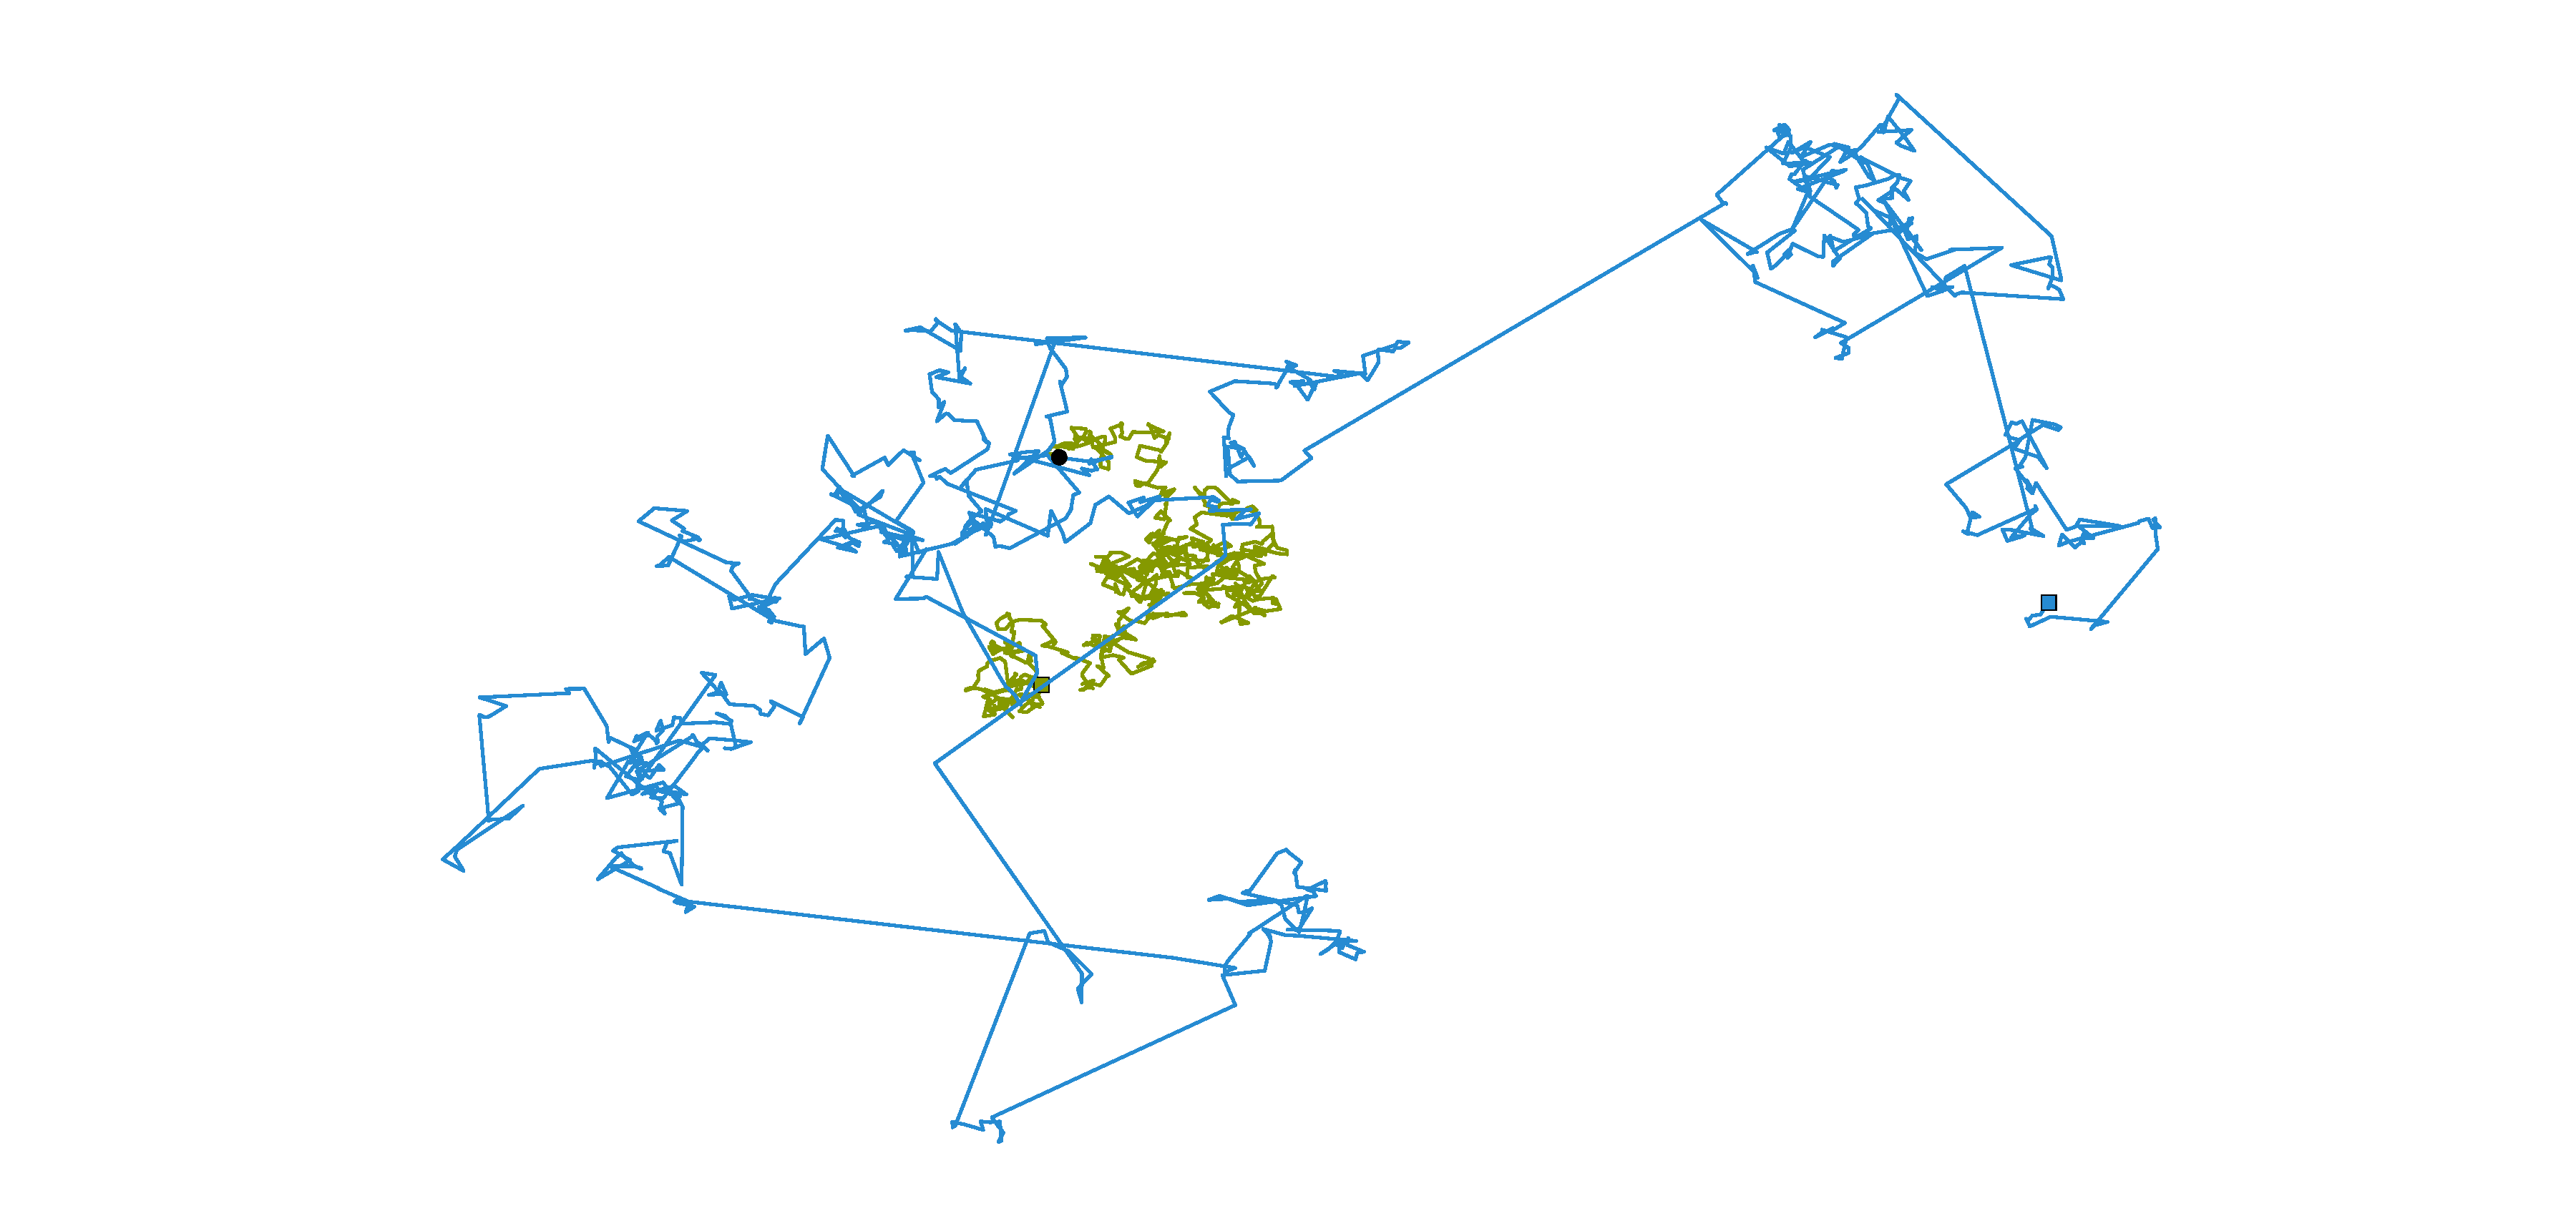
\includegraphics{LevyFlight/levy_vs_gaussian.pdf}
    \end{center}
    \caption{Mouvement brownien (en vert) et vol de Lévy (en bleu) pour 200 pas aléatoires.
             \label{fig:levy_vs_gaussian}}
\end{figure}
\FloatBarrier
% subsubsection vol_de_levy (end)


% - - - - - - - - - - - - - - - - - - - - - - - - - - - - - - - - - - - - - - -
\subsubsection{Apprentissage par Vecteur opposée} % (fold)
\label{ssub:apprentissage_par_vecteur_opposee}
Les méthodes d’optimisation et spécifiquement les approchées sont fortement
dépendantes de la population initiale (\mtodo{Ajouter source}). Il est ainsi nécessaire
de constituer une population couvrant de manière homogène l’espace de décision.
L’approche la plus répandu est d’initialiser la population initiale suivant une
distribution uniforme suivant \eqref{alg:init_phase}.
Afin d’améliorer la diversité sans connaissances a priori,\cite{Tizhoosh2005695}
développe l’Opposite Based Learning (OBL) (Définition~\ref{def:oblm}).

\begin{Def}[OBL~:~Apprentissage par vecteur opposé]\label{def:oblm}
Admettons un point de dimension $D$, $\vec{x}(x_{1}, x_{2}, ..., x_{D})$ avec
$x_{1}, x_{2}, ..., x_{D}$ des valeurs bornées. Si $x_{i} \in [a_{i}, b_{i}]$ pour
$i = 1, 2, ..., D$ alors le point opposée est $\vec{\check{x}}(\check{x_{1}}, \check{x_{2}}, ..., \check{x_{D}})$ est définie par:
\[\check{x_{i}} = a_{i} + b_{i} - x_{i}\]
\end{Def}

\cite{Rahnamayan2008906} l’adapte pour l’algorithme Differential evolution (DE)
et montre que la probabilité d’améliorer une solution est plus grande
avec sa position opposée que avec une nouvelle position aléatoire.
Il l’utilise pour l’initialisation et aussi durant l’optimisation. Les bornes
($a_{i}$ et $b_{i}$) sont alors définies dynamiquement afin d’éviter de ralentir la convergence.
Cette approche a aussi été appliquée avec succès dans le cas de l’algorithme ABC en couplage
avec un opérateur de mutation \parencite{Bi2011174} ou encore en coopération avec une marche
aléatoire \parencite{Sharma2012213}.
Il a aussi été appliqué pour résoudre des problèmes à objectifs multiples,
en combinaison avec un algorithme évolutionnaire \parencite{Ma201448}, ou encore avec le PSO \parencite{Gao2013114}.

L’approche est ainsi retenue afin d’améliorer la diversité de la population initiale
et sera aussi utilisé durant la phase des exploratrices permettant d’augmenter l’exploration.
Pour chaque source, une position candidate ($\vec{x}$) et son opposée ($\vec{\check{x}}$) sont évaluées.
Un tournoi binaire est alors organisé et seule la meilleure solution est conservé comme source.
% subsubsection apprentissage_par_vecteur_opposee (end)


% - - - - - - - - - - - - - - - - - - - - - - - - - - - - - - - - - - - - - - -
\subsubsection{L’$\epsilon$-dominance} % (fold)
\label{ssub:epsilon_dominance}
Contrairement à une approche mono objectif, il existe plusieurs solutions optimales.
Il est alors nécessaire de conserver l’évolution du front de Pareto à travers une
archive (\mtodo{Lien vers figure}).

\ftodo{Ajouter graphe décrivant l’utilité de l’archive pour la recherche \cite{Laumanns2002263}}

Afin de garantir la convergence il est nécessaire d’utiliser une approche élitiste
en limitant la taille de l’archive au solution les plus performantes afin d’éviter
une convergence trop lente \parencite{Zitzler2000173}. De plus afin d’éviter de converger vers un front local,
il est nécessaire de maintenir de la diversité dans la population.
Dans les approches couramment utilisées on peut citer le Fast Non Dominated Sorting Algorithm utilisé dans la version
de base du NSGA-II \parencite{Deb2002182}. Dans cette approche une sélection par rang
est appliqué permettant de trier le front en différents niveaux et la distance dite
de crowding (distance moyenne entre deux solutions) est utilisée afin de maintenir la diversité.
L’algorithme SPEA II améliore la diversité du front final au prix d’une convergence
plus lente en utilisant une approche par clustering. $N$ clusters (taille de l’archive)
sont formés en se basant sur la distance euclidienne et une solution par cluster
est retenue.
\cite{Laumanns2002263} propose de séparer l’espace des solutions en une grille en ajoutant la notion
de $\epsilon$-dominance. Dans cette approche l’espace des objectifs est divisé en hypercubes,
et chaque hypercube est comparé selon l’$\epsilon$-dominance (Définition~\ref{def:eps_dominance}).
Bien que d’autres approches utilisent une grille similaire (PAES, \cite{Knowles2000149}
l’$\epsilon$-dominance n’accepte qu’une unique solution par hypercube assurant une
plus grande diversité de la population. La taille de l’archive est donc fonction
des $\epsilon$ choisis pour chaque objectif mais est toujours finie.


\begin{Def}[$\epsilon$-dominance]\label{def:eps_dominance}
L’$\epsilon$-dominance assume que deux solutions sont identiques lorsqu’elles appartiennent
au même hypercube dont les dimensions des arrêtes sont définies par $\vec{\epsilon}_{i}, i \in \{1, ..., M\}$ avec $M$ le nombre
de fonction objectif.
Dans le cas d’une maximisation il est dit que $\vec{x}_{a}$ $\epsilon$-domine $\vec{x}_{b}$ si :
\begin{align*}
  \forall j \in \{1, M\}, \qquad \left\lceil\frac{f_{j}(\vec{x}_{a})}{\epsilon}\right\rceil &\leq \left\lceil\frac{f_{j}(\vec{x}_{b})}{\epsilon}\right\rceil  \\
  \intertext{et}
  \exists i \in \{1, M\}, \qquad \left\lceil\frac{f_{i}(\vec{x}_{a})}{\epsilon}\right\rceil &< \left\lceil\frac{f_{i}(\vec{x}_{b})}{\epsilon}\right\rceil  \\
\end{align*}
Cette relation sera notée sera notée : $\vec{x}_{a} \prec_{\epsilon} \vec{x}_{b}$.
\end{Def}

Une solution peut ainsi être ou dominée, dominante, identique, ou non-dominée au
sens de l’$\epsilon$-dominance, les solutions $\epsilon$-non-dominées formant alors
le front d’$\epsilon$-Pareto (Fig.~\ref{fig:epsilon_dominance}).
Dans un premier temps les solutions sont alors départagées selon l’$\epsilon$-dominance.
Dans le cas où une nouvelle solution serait $\epsilon$-identique elle est uniquement
comparée avec celle déjà archivée dans le même hypercube en utilisant la distance euclidienne.
Afin d’éviter l’ajout de biais, les objectifs sont normalisés en fonction des dimensions
de l’hypercube.
Ensuite dans le cas d’une maximisation la solution retenue est celle la plus proche
du maximum de l’hypercube. Contrairement à une sélection par dominance stricte le
calcul de la distance euclidienne permet de tenir compte de l’ensemble des amélioration
en étant moins élitiste.
L’$\epsilon$-archive permet ainsi d’assurer :
\begin{itemize}
  \item L’élitisme : seule les solutions non-dominées sont retenues
  \item La diversification : une unique solution par hypercube
  \item Une taille limite : La taille maximale est fonction des $\epsilon$ et finie
  \item Une intensification : En réduisant les $\epsilon$ on augmente la taille maximale
  \item Une épuration : En augmentant les $\epsilon$ on réduit la taille maximale
\end{itemize}

\begin{figure}
    \begin{center}
        \includegraphics{abc/selection_boxes.png}
    \end{center}
    \caption{Principe de la mise à jour de l’archive par epsilon-dominance (maximisation assumée).
             Adapté de \cite{Deb2005501}.
             \label{fig:epsilon_dominance}}
\end{figure}

L’étude réalisé par \cite{Deb2005501} montre que cette méthode d’archivage permet
d’obtenir une très bonne convergence et une grande diversité sur le front final. Les résultats
indiquent que les approches PESA et NSGA II obtiennent une moins bonne représentation
du front de Pareto que celles utilisant le clustering (C-NSGA II, SPEA) et l’$\epsilon$-dominance ($\epsilon$-MOEA).
Cette observation est d’autant plus vrai pour des problèmes ayant 3 objectifs (DTLZ1, ..., DTLZ7).
De plus les résultats mettent aussi en évidence que le NSGA II et le $\epsilon$-MOEA
converge plus rapidement que le SPEA II.
Un désavantage de cette méthode peut cependant être noté. De part sa formulation
les solutions au niveau des extrêmes sur le front de Pareto sont plus difficilement
atteignable.

L’$\epsilon$-archive est donc retenue comme solution d’archivage dans ces travaux
car il représente un bon compromis entre diversité et convergence.
% subsubsection epsilon_dominance (end)


% - - - - - - - - - - - - - - - - - - - - - - - - - - - - - - - - - - - - - - -
\subsubsection{Prise en compte des contraintes :} % (fold)
\label{ssub:prise_en_compte_des_contraintes}
Les problèmes multi-objectif dans le domaine de l’ingénierie sont souvent
dépendantes de contraintes limitant l’ensemble des solution optimales au domaine
de faisabilité. L’optimisation consiste alors à améliorer les objectifs tout en
respectant les contraintes spécifiques au problème \eqref{eq:def_optimisation}.

La littérature introduit de nombreuses variation permettant de tenir compte des
contraintes. L’approche la plus courante est d’utiliser un facteur de pénalité.
Ce facteur est dit statique si il est fixe durant l’ensemble de l’optimisation, dynamique
si il est adapté en fonction du nombre d’itération, et adaptatif si les informations
acquises par la recherche aide à sa détermination \parencite{Coello2002}.
Parmi les approches existante il peut être cité la méthode de la peine de mort
qui consiste à appliquer une pénalité très importante afin de rejeter les solutions
sous contraintes. D’autres moins exclusives désavantagent les solutions ne respectant
pas les contraintes en fonction du niveau de violation des contraintes. D’autres approches
ajustent dynamiquement la pénalité en fonction des itération de l’algorithme. Le
problème récurrent avec ces approches réside dans l’ajout de paramètres supplémentaires
devant être déterminés empiriquement.

\cite{Coello2002} explique qu’une bonne prise en compte des contraintes ne devraient
pas nécessité le paramétrage de facteurs. Il explique aussi que ces facteurs impactent
fortement la performance de la méthode de prise en compte des contraintes. De plus
la méthode sélectionnée ne devrait pas demandé un nombre plus important d’évaluation
qui peuvent être très couteuses. \cite{Deb2000311} propose une méthode de
sélection par tournoi dont les règles sont les suivantes :
\begin{itemize}
  \item Une solution avec contraintes est inférieure à une solution sans contraintes
  \item Si les deux solutions sont sans contraintes la solution dominante est préférée
  \item Si les deux solutions sont sous contraintes, la solution violant le moins les contraintes est préférée
\end{itemize}
La méthode a l’avantage d’être simple à mettre en place et est utilisé pour de nombreux
cas d’application (\mtodo{Ajouter des ref dans le bâtiment}). La méthode est cependant
très élitiste car les solutions non faisables sont toujours écartées durant la
recherche.

Dans ces travaux, une méthode adaptative moins élitiste est retenue. Adaptée
aux problèmes multi-objectif par \cite{Woldesenbet20073077}, la méthode ne demande
aucun paramétrage, et l’objectif modifié est calculé de la manière suivante :
\begin{itemize}
  \item Normaliser les objectifs selon \eqref{eq:norm_obj}
  \item Normaliser les contraintes et les agréger pour former une unique contrainte selon \eqref{eq:norm_contrainte}
  \item Calculer les objectifs modifiés par agrégation des contraintes et des objectifs selon \eqref{eq:calc_modif_obj}
\end{itemize}

\begin{align}\label{eq:norm_obj}
  \tilde{f}_{i}(\vec{x}) &= \begin{cases}
    \frac{f_{i}(\vec{x}) - min(f_{i}(\vec{x}))}{max(f_{i}(\vec{x})) - min(f_{i}(\vec{x}))} & \text{(minimisation)} \\ \\
    1 - \left[\frac{f_{i}(\vec{x}) - min(f_{i}(\vec{x}))}{max(f_{i}(\vec{x})) - min(f_{i}(\vec{x}))}\right] & \text{(maximisation)} \\
  \end{cases}
\end{align}
avec $f_{i}(\vec{x})$ la valeur de l’objectif $i$, pour la position $\vec{x}$ dans l’espace de décision.
\iunsure{Détailler pourquoi différence entre max et min}

\begin{equation}\label{eq:norm_contrainte}
  v(\vec{x}) = \frac{1}{J+K} \sum_{j=1}^{J+K} \frac{g_{j}(\vec{x})}{max(g_{j}(\vec{x}))}
\end{equation}
avec $J$ le nombre de contraintes d’inégalités et $K$ le nombre de contrainte d’égalités
transformées en contraintes d’inégalités. $g_{j}$ représente alors la fonction contrainte
associée à la contrainte $j$ avec $g_{j} \geq 0$.

\begin{equation}\label{eq:calc_modif_obj}
  F_{i}(\vec{x}) = d_{i}(\vec{x}) + p_{i}(\vec{x})
\end{equation}
avec $d_{i}(\vec{x})$ calculé selon \eqref{eq:dist_obj} et $ p_{i}(\vec{x})$ selon \eqref{eq:penalty_norm}.


\begin{align}\label{eq:dist_obj}
  d_{i}(\vec{x}) = \begin{cases}
                          v(\vec{x})                                     & \qquad si\  r_{f} = 0 \\
                          \sqrt{v(\vec{x})^2 + \tilde{f}_{i}(\vec{x})^2} & \qquad sinon          \\
                    \end{cases}
\end{align}
\begin{equation}\label{eq:penalty_norm}
  p_{i}(\vec{x}) = (1 - r_{f})  X(\vec{x}) + r_{f} Y_{i}(\vec{x}) \\
\end{equation}

\begin{align*}
  \shortintertext{où} \\
    r_{f} &= \frac{\text{Nombre de solution réalisables}}{\text{Taille de la population}} \\
  \shortintertext{et} \\
  X(\vec{x})     &= \begin{cases}
                0,          \qquad     & si\  r_{f} = 0\\
                v(\vec{x}), \qquad     & sinon\\
                \end{cases} \\
  Y_{i}(\vec{x}) &= \begin{cases}
                    0,          \quad \qquad & \text{si} \ \forall j, \ g_{j}(\vec{x}) = 0\\
                      \tilde{f}_{i}(\vec{x})  \\
            \end{cases}\\
\end{align*}

L’algorithme s’adapte ainsi dynamiquement à la population et peut accepter des
solutions ne respectant pas les contraintes. Plus il y a de solutions non
réalisables dans la population, moins une solution ne respectant pas les contraintes à
de chances d’être sélectionnée. L’approche permet d’améliorer l’exploration de
l’espace de décision et ainsi de pouvoir trouver des solutions existantes même
lorsque l’espace de faisabilité est faible.
L’approche est donc retenue dans ces travaux mais uniquement utilisée lors de la mise à jour
des solutions de la population. L’archive elle, n’accepte que des solutions respectant les
contraintes.
% subsubsection prise_en_compte_des_contraintes (end)


% - - - - - - - - - - - - - - - - - - - - - - - - - - - - - - - - - - - - - - -
\subsubsection{Description globale de l’approche} % (fold)
\label{ssub:description_globale_de_l_approche}
Dans la section précédente, chaque élément utilisé dans l’algorithme a été détaillé et
les avantages et inconvénients des approches retenues ont aussi été explicités.
Dans cette section le fonctionnement global de la méthode approchée d’optimisation
multi-objectif retenue est décrite.

\begin{figure}
    \begin{center}
        \includegraphics[width=10cm]{abc/algorithme_complet.pdf}
    \end{center}
    \caption{Description globale de l’algorithme ABC pour les problèmes multi-objectif.
             \label{fig:abc_complet}}
\end{figure}

L’algorithme peut être définie par Fig.~\ref{fig:abc_complet}.
Les sources sont initialisées (Algorithm~\ref{alg:init_phase}) suivant la méthode
OBL (Définition~\ref{def:oblm}) afin d’obtenir une meilleure représentation du
domaine de décision en amont de l’optimisation.
Durant la phase des butineuses (Algorithm~\ref{alg:employed_phase}), chaque source
subit une variation en tenant compte de deux sources, une de l’essaim et une de l’archive.
Durant la phase des ouvrières (Algorithm~\ref{alg:onlooker_phase}), la qualité de
chaque source \eqref{eq:attribution_prob_to_source} est utilisée afin de sélectionner
et d’exploiter seulement les plus prometteuses. Finalement, si une source a subit le
nombre maximum d’échec ($MaxEchec$) alors une exploratrice (Algorithm~\ref{alg:scout_phase})
réinitialise sa position de manière aléatoire.
Tant que la condition d’arrêt n’est pas atteinte, les phases des butineuses,
des ouvrières, et des exploratrices sont répétées de manière cyclique. Au cours de
la recherche les nouvelles sources sont ajoutées à l’archive qui seront ensuite utilisées
comme élément d’apprentissage pour les butineuses et les ouvrières mais pas pour les
exploratrices. Une fois la condition d’arrêt atteinte l’ensemble des solutions
de l’archive forment le front de Pareto.

Dans l’optique de l’optimisation d’un modèle solaire développé sous Dymola, l’algorithme
a été implémenté en \emph{Python} afin de faciliter le couplage avec la bibliothèque
\emph{BuildingsPy} qui comme nous l’avons vu dans le chapitre précédent permet d’automatiser
la simulation de modèle \emph{Modelica} sous \emph{Dymola}. La bibliothèque est
disponible sous le nom de \emph{pyMOABC} et implémente :
\begin{itemize}
  \item une $\epsilon$-archive et la box-dominance
  \item la dominance au sens de Pareto
  \item la prise en compte des contraintes suivant \cite{Woldesenbet20073077}
  \item une interface commune permettant l’abstraction du type de variable (discrète, continue, qualitative)
  \item une représentation des solutions (sources et abeilles)
  \item l’algorithme tel que décrit dans ces travaux
  \item une suite de test pour des optimisation avec ou sans contraintes
\end{itemize}

L’approche retenue contrairement à la majorité des méta-heuristiques est robuste et demande
peu de paramètre à définir de manière empirique. En effet seul la taille de la population
et le nombre d’essai maximum sont à définir. De plus la taille de la population
n’impacte pas le nombre de solutions dans l’archive car le stockage est réalisé dans
une structure indépendante. Il est aussi important de noter que ces deux paramètres
on un comportement prévisible facilitant leur paramétrage. La
taille de la population en augmentant améliore l’exploration réduisant le risque
de se bloquer dans les optimums locaux mais réduit la vitesse de convergence (Définition~\ref{def:convergence}).
Le nombre d’essai maximum lui est directement lié au nombre de critères variant
dans l’espace de décision et à la taille de la population. Une valeur faible traduisant
l’abandon rapide d’une solution. Ainsi on note clairement que la taille de la population
impacte fortement l’exploration là où le nombre d’essai maximum impacte l’exploitation.

% Phase d’initialisation
\begin{algorithm}\label{alg:init_phase}
  \SetAlgoVlined
  \DontPrintSemicolon
  \emph{Initialisation des \ASources sur l’ensemble de l’espace de décision}\;
  \For{$i \leftarrow 0$ \KwTo \ANbrSources}
  {
    \emph{Initialisation des critères pour chaque source}\;
    \For{$j \leftarrow 0$ \KwTo \ANbrCriteria}
    {
      \encircle{a} \emph{Initialisation de la position de la $\ASource_{i}$ de manière aléatoire}\;
      \Indp
      $x_{ij} = x_{j}^{min} + RandUniform(0, 1) \times (x_{j}^{max} - x_{j}^{min})$\;
      \Indm
      \BlankLine
      \encircle{b}  \emph{Génération de l’$\ABee_{i}$ dont la position est générée suivant Définition~\ref{def:oblm}}\;
      \Indp
      $ \check{x_{ij}} = x_{j}^{min} + x_{j}^{max} - x_{ij}$\;
      \Indm
      \BlankLine
      \encircle{c} \emph{Évaluation de la $\ASource_{i}$ et de l’$\ABee_{i}$}\;
      \BlankLine
      avec $RandUniform$ un tirage aléatoire suivant une loi uniforme, et $x_{j}^{min}$, $x_{j}^{max}$
      respectivement le minimum et le maximum du critère $j$\;
    }
    \If{$\ASource_{i}$ respecte toutes les contraintes}
    {
      $\AArchive \pluseq \ASource_{i}$ \AComment{On ajoute la source initial à l’archive}
    }
    \If{$\ABee_{i}$ respecte toutes les contraintes}
    {
      $\AArchive \pluseq \ABee_{i}$ \AComment{On ajoute la source opposée à l’archive}
    }
  }
  Mise à jour des \ASources d’après Algorithm~\ref{alg:maj_phase}\;
  \caption{Initialisation des sources par OBLM (Définition~\ref{def:oblm}).}
\end{algorithm}

% Phase des éclaireuses
\begin{algorithm}\label{alg:scout_phase}
  \SetAlgoVlined
  \DontPrintSemicolon
  \AComment{Exploration par les \AScouts}
  \For{$i \leftarrow 0$ \KwTo \ANbrSources}
  {
    \If{$\ATrial_{i} > \AMaxTrial$ }
    {
      Génération de deux nouvelles positions suivant Algorithm~\ref{alg:init_phase}\;
    }
  }
  Mise à jour de la position des \ASources d’après Algorithm~\ref{alg:maj_phase}\;
  \caption{Phase des éclaireuses.}
\end{algorithm}


% Phase des ouvrières
\begin{algorithm}\label{alg:onlooker_phase}
  \SetAlgoVlined
  \DontPrintSemicolon
  \AComment{Exploitation des sources par les \AOnlookers}
  \AComment{Plusieurs \AOnlookers peuvent modifier la même source}
  \For{$\AOuvriere \in \AOnlookers$}
    {
      Sélection aléatoire d’une \ASource $i$ selon la probabilité
      définie par l’équation \eqref{eq:attribution_prob_to_source}\;
      Sélection aléatoire d’une source $k$ ($k \neq i$) dans l’\AArchive\;
      \encircle{a} \emph{Génération d’une nouvelle position $\check{\vec{x_{i}}}$ à partir de la
                         position $\vec{x_{i}}$ pour l’\AOuvriere }\;
      \For{$j \leftarrow 0$ \KwTo \ANbrCriteria}
      {
      \begin{algomathdisplay}
        \check{x_{ij}} =%
          \begin{cases}
            x_{ij}  + RandUniform(-1, 1)   \times \ (x_{ij} - x_{kj}) &\ \ATirageB < \AMR \\
            x_{ij}                                                    &\ sinon
          \end{cases}
      \end{algomathdisplay}
      }
      \BlankLine
      Avec \AMR est la probabilité de réaliser une modification (fixée à 0,5) et
      \ATirageB un nombre aléatoire entre 0 et 1\;
      \BlankLine
      \encircle{b} \emph{Évaluation des objectifs pour la nouvelle position $\check{\vec{x_{i}}}$}\;
      \BlankLine
      \If{\AOuvriere respecte toutes les contraintes}
      {
        $\AArchive \pluseq \AOuvriere$ \AComment{Ajout de la solution trouvée par l’\AOuvriere à l’archive}
      }
    }

  Mise à jour de la position des \ASources qui ont été modifiées d’après Algorithme~\ref{alg:maj_phase}\;
  \caption{Phase des ouvrières.}
\end{algorithm}

% Maj des sources
\begin{algorithm}\label{alg:maj_phase}
  \SetAlgoVlined
  \DontPrintSemicolon
  Récupérer le maximum et minimum pour chaque objectif dans l’\AHive\;
  Récupérer le maximum pour chaque contrainte dans l’\AHive\;
  \For{$\ABee \in \ABees$}
  {
    Calcul du vecteur objectif pour l’\ABee ($\check{\vec{F}}_{i}$) et pour sa \ASource $i$ ($\vec{F}_{i}$),
    respectivement aux positions $\check{\vec{x_{i}}}$ et $\vec{x_{i}}$
    selon \eqref{eq:calc_modif_obj}\;
    \For{$m \leftarrow 1$ \KwTo M}
    {
      \begin{algomathdisplay}
      \begin{aligned}
      \check{F}_{im} &= d_{m}(\check{\vec{x_{i}}}) + p_{m}(\check{\vec{x_{i}}}) \\
      F_{im}         &= d_{m}(\vec{x_{i}}) + p_{m}(\vec{x_{i}}) \\
      \end{aligned}
      \end{algomathdisplay}
    }
    \If{$\check{\vec{x_{i}}} \succ \vec{x_{i}}$}
    {

      $\ASource_{i} \leftarrow \ABee$ \AComment{Mise à jour de la \ASource à partir de l’\ABee}

      $\ATrial_{i} \leftarrow 0$ \AComment{On réinitialise le nombre d’essais pour la \ASource $i$}
    }
    \Else
    {
      $\ATrial_{i} \pluseq 1$ \AComment{On incrémente le nombre d’essais pour la \ASource $i$}
    }
  }
  \caption{Mise à jour des \textbf{Sources} par les \textbf{Abeilles}}
\end{algorithm}

% Phase des butineuses
\begin{algorithm}\label{alg:employed_phase}
  \SetAlgoVlined
  \DontPrintSemicolon
  \AComment{Exploration des sources par les \AEmployed}
  \For{$i \leftarrow 0$ \KwTo \ANbrSources}
  {
    Sélection aléatoire d’une source $k$ ($k \neq i$) dans l’\AArchive\;
    Sélection aléatoire d’une source $p$ ($p \neq i$) dans l’\AHive\;
    \BlankLine
    \encircle{a} \emph{Génération d’une nouvelle position $\check{\vec{x_{i}}}$ à partir de la %
                       position $\vec{x_{i}}$ pour la \AButineuse $i$}\;
    \If{$\ATirageA < \ARatio $ }
      {
      \For{$j \leftarrow 0$ \KwTo \ANbrCriteria}
      {
      \begin{algomathdisplay}
        \check{x_{ij}} =%
          \begin{cases}
            \begin{aligned}
              x_{ij}  &+ 0.01 \times  \ALevy  &\times \ (x_{ij} - x_{pj})  \\
                      &+ 0.01 \times |\ALevy| &\times \ (x_{kj} - x_{ij})  \\
            \end{aligned} &\ \ATirageB < \AMR \\
            x_{ij}        &\ sinon
          \end{cases}
      \end{algomathdisplay}
      \ALevy est nombre aléatoire dans une distribution de Lévy
      permettant de réaliser un vol de Lévy (Définition~\ref{def:vol_levy})\;
      }
      }
    \Else
      {
      \For{$j \leftarrow 0$ \KwTo \ANbrCriteria}
      {
      \begin{algomathdisplay}
        \check{x_{ij}} =%
          \begin{cases}
            \begin{aligned}
              x_{ij}  &+ RandUniform(-1, 1)   &\times \ (x_{ij} - x_{pj})  \\
                      &+ RandUniform(0, 1)    &\times \ (x_{kj} - x_{ij})  \\
            \end{aligned} &\ \ATirageB < \AMR \\
            x_{ij}        &\ sinon
          \end{cases}
      \end{algomathdisplay}
      }
      }
      Où \ARatio est la probabilité de réaliser un vol de Lévy (fixée à 0,5), et \AMR la probabilité
      de réaliser une modification (fixée à 0,8). \ATirageA et \ATirageB étant des nombres aléatoires
      (entre 0 et 1) tirés dans une distribution uniforme\;
      \BlankLine
    \encircle{b} \emph{Évaluation des objectifs pour la nouvelle position $\check{\vec{x_{i}}}$}\;
    \If{$\AButineuse_{i}$ respecte toutes les contraintes}
    {
      \AComment{On ajoute la nouvelle source à l’archive}
      $\AArchive \pluseq \AButineuse_{i}$\;
    }
  }
  \AComment{On ne conserve que une seule position par source}
  Mise à jour de la position des \ASources d’après Algorithme~\ref{alg:maj_phase}\;
  \caption{Phase des butineuses.}
\end{algorithm}

\FloatBarrier
% subsubsection description_globale_de_l_approche (end)


% - - - - - - - - - - - - - - - - - - - - - - - - - - - - - - - - - - - - - - -
\subsubsection{Validation par étalon} % (fold)
\label{ssub:validation_par_etalon}

Cette section permet d’apprécier la performance de l’approche pour différent types
de problèmes pouvant être rencontrés dans un problème d’optimisation.

\itodo{Cette section est en construction}

Premièrement la convergence vers le front de Pareto a été vérifié à travers de nombreux
problèmes d’optimisation multi-objectif comportant ou non des contraintes.
Dans cette optique la bibliothèque \emph{pyMOABC} a été développée autour de tests unitaires
(Test-driven development).
Chaque éléments (fonction / méthodes / ...) et comportements (minimisation / maximisation / ...)
ont ainsi été testés afin de garantir que la bibliothèque implémente correctement
les éléments et comportements nécessaires. De plus une fois le test réussi son existence
permet de garantir que les modifications futures respecteront l’ensemble des contraintes
déjà existantes.
Cette approche couplée aux problèmes étalon existants a ainsi permit de valider
l’implémentation de l’approche.
Deuxièmement bien que la réussite d’un problème étalon ne suffise à garantir la
convergence sur un problème réel, il apporte une information importante : la capacité
du méta-heuristique à résoudre ce type de problèmes. Dans cette optique les résultats
qui seront présentés dans cette section sont sélectionnés afin d’évaluer la performance
de l’algorithme sur des étalons \ftodo{trouvé mieux}{variés}.

Les problèmes retenus sont ainsi les suivants :
\begin{itemize}
  \item front convexe : ZDT1 (2 objectifs)
  \item front concave : ZDT2 (2 objectifs)
  \item multi-modal : ZDT4 (2 objectifs)
  \item Non-uniformité avec faible densité près de l’optimal : DTLZ5, ZDT6, ConvexGlobalNonConvexLocalHive
  \item Discontinue : DTLZ6, Kursawe
\end{itemize}


\itodo{Je suis ici !}

% subsubsection validation_par_etalon (end)
% section construction_d_un_meta_heuristique_adapte (end)


% subsubsection principe_de_fonctionnement (end)
% subsection artificial_bee_colony (end)
% % À mettre ailleurs
% Ensuite il est nécessaire que l’approche soit simple à coupler avec les outils
% utilisés. La restriction principale étant le couplage avec le logiciel Dymola.
% Comme il a été décrit dans le chapitre précédent, un outil a été développé sur la
% base de la bibliothèque BuildingsPy afin de simuler de manière concurrente le modèle.
% Afin de profiter de ces outils, seul les solutions développées en Python et donc
% simplement interfaçable avec les outils précédent sont retenus.
% DEAP (\mtodo{Ajouter source}) est une bibliothèque Python développée afin de
% permettre la construction de méta-heuristiques. Il est construit de manière à
% permettre à l’utilisateur de se concentrer sur la formulation du problème et
% faire abstraction des structures nécessaires. Il fournit ainsi les briques
% nécessaires à la construction de différents méta-heuristique et propose des
% exemples d’implémentation d’algorithmes évolutionnaires.
% Ce bibliothèque ne sera finalement pas utilisée pour plusieurs raisons.
% \begin{itemize}
%   \item Les structures de données nécessaires à l’approche retenue
%         ne sont pas disponibles
%   \item La bibliothèque ne propose pas de solution pour gérer la mixité des
%         critères de décisions
%   \item Pas de support pour les marches aléatoires
% \end{itemize}
% subsection choix_du_générateur (end)

% % ------------------------------------------------------------------------------
% \subsection{Introduction} % (fold)
% \label{sub:introduction}
% \itodo{À reprendre complètement}

% L’optimisation multi-objectif est aujourd’hui largement utilisé dans le bâtiment.
% On a par exemple \cite{Armand-Decker2015} qui a développé une méthode d’optimisation pour les
% construction bois en utilisant un meta-modèle de bâtiment. Elle utilise un meta-heuristique
% à population (Particule Swarm optimization) et évalue les besoins en énergie, le confort des
% occupants, la sécurité de l’ouvrage et de l’impact environnemental. \cite{Rivallain2013}
% a quand à lui utilisé une méthode approchée (NSGA-II) et une exacte (programmation dynamique)
% pour identifier des programmes séquentiels efficaces de réhabilitation énergétique.
% Il a ainsi optimisé la combinaison des modifications pour chaque phase mais aussi l’ordre
% dans lequel ces améliorations doivent être réalisées afin d’être le plus optimal
% possible.
% Pour les différentes solutions l’impact environnemental, le confort des occupants en
% période estivale, et le coût ont été évaluées.
% \itodo{Ajouter des sources vers des exemples d’optimisation de bâtiment}

% On a aussi de nombreux exemples d’optimisation de système énergétique.
% \itodo{Ajouter des sources vers des exemples d’optimisation de système}

% On voit donc que l’optimisation est un outil qui a été largement utilisé dans
% le bâtiment comme pour l’amélioration ou l’identification de solutions performantes
% pour les systèmes.

% \itodo{Ajouter du bla bla sur l’originalité et les perspectives de ces travaux}
% L’originalité de ce travail provient principalement du couplage entre le bâtiment
% et ses systèmes. La plupart des optimisations de bâtiment évalues les besoins
% du bâtiment et considère donc un système de chauffage et de ventilation idéaux.
% Dans ces travaux on cherche à optimiser la partie système et son algorithme de
% contrôle en même temps que l’enveloppe du bâtiment. On évalue donc plus un besoin
% en énergie mais une consommation qui est fonction de la performance des systèmes
% envisagées. Les travaux se concentre sur l’évaluation de solutions utilisant fortement
% l’énergie solaire comme vecteur énergétique. On cherche donc à couvrir les besoins
% de chauffage, d’eau chaude sanitaire (ECS) et d’électricité.
% Cette approche permettra d’évaluer le potentiel d’autonomie solaire disponible
% pour différentes combinaisons systèmes/enveloppe.

% Enfin ces travaux vise à l’élaboration d’un outil d’aide à la décision. Il existe
% diverses methodes pour faire de l’aide à la décision (~\autoref{sec:vers_une_optimisation_multi_critere_et_multi_objectif}).
% L’approche choisie est de déterminer un
% ensemble de solutions non-dominées dans un premier temps, puis d’utiliser des
% outils d’aide à la décision pour réduire le nombre de solution. On se trouve donc
% dans une approche par front de Pareto.
% \itodo{Ajouter du bla bla sur le choix de l’ordre entre optimisation et aide à la décision}

% \itodo{Reformuler tout ça pour mieux introduire les parties qui suivent}
% % subsection introduction (end)
% % subsection les_approches_existantes (end)
% % section vers_une_optimisation_multi_critere_et_multi_objectif (end)






% \paragraph{Convergence} % (fold)
% \label{par:convergence}
% \itodo{Décrire convergence}
% % paragraph convergence (end)

% \paragraph{Diversité} % (fold)
% \label{par:diversité}
% \itodo{Décrire diversité}
% % paragraph diversité (end)


% % ..............................................................................
% % ..............................................................................
% \section{Construction d’un outil d’aide à la décision} % (fold)
% \label{sec:construction_d_un_outil_d_aide_à_la_decision}


% % ------------------------------------------------------------------------------
% \subsection{Génération de solutions: quelle méthode ?} % (fold)
% \label{sub:generation_de_solutions_quelle_methode}
% % Description du Meta-heuristique choisi:
% %  - Origine de l’algorithme (inspiration des abeilles):
% % Décrire l’origine de cet algorithme. Décrire les recherches qui ont été faites sur
% % les abeilles et ensuite les conclusions tirées par l’inventeur pour formuler ce
% % meta-heuristique.
% % Les sources suivantes non pas encore été lues: \cite{Camazine1991547}, \cite{Seeley1996}
% % mais traitent du comportement des abeilles.
% %  - Formulation théorique:
% %     + Description des différentes étape de résolution de la méthode:
% %       Détails pour onlookers, employed, scout, ...
% %       Détails pour les paramètres nécessaires au fonctionnement de l’heuristique.
% %     + Description de la mise à jour de la position d’une source:
% %       Dans le cas de variables continues la formulation de base est applicable et sera
% %       donc conservée. Dans le cas de variables discrètes on utilisera une méthode alternative
% %       développée dans `10.1177/0021998308097681` et `tel-01234197, version 1`.

% % - - - - - - - - - - - - - - - - - - - - - - - - - - - - - - - - - - - - - - -
% \subsubsection{Quelle approche d’optimisation ?} % (fold)
% \label{ssub:quelle_approche_d_optimisation_}
% Comme nous l’avons vu précédemment, il existe de nombreux meta-heuristiques dans
% la littérature. Cependant il n’existe pas à la connaissance de l’auteur de méthode
% pour sélectionner un algorithme qui sera le plus performant pour un problème donnée.
% Ce principe a été formalisé par \cite{Wolpert199767} \itodo{Pas encore lu ...}. Il démontre qu’il
% n’y a aucunes \emph{à priori} différences entre les algorithmes. Les critères
% permettant de sélectionner un meta-heuristique sont donc à caractère subjectif.
% Un des arguments pertinent qui peut être mis en avant est le nombre de paramètres
% nécessaires pour le réglage de l’algorithme. En effet sur ce point les algorithmes
% sont très différents, certains demandant de nombreux paramètres à configurer
% \itodo{Citer des exemple de algo génétique, réseaux de neuronnes, ...} contrairement
% à d’autres \itodo{Citer des exemples de PSO, ABC, ...}. Un autre critère pertinent
% est la robustesse des algorithmes. On entend par \emph{robuste} la capacité des algorithmes
% à converger pour différentes valeurs de paramètre. Par exemple le meta-heuristique PSO
% peut être considérée comme robuste \itodo{Mettre des sources} car la solution n’est
% pas fortement influencée par le choix de la configuration.
% À l’opposée des approches par réseau de neurones \itodo{Mettre des sources} sont
% très sensibles, et la variation d’un paramètre peut donner une solution complètement
% différente (pour le meilleur et le pire).
% Afin de pallier à ces problème, des outils existent pour paramétrer ces meta-heuristique.
% C’est particulièrement vrai dans le cas d’optimisation mono-critère mais commence
% aussi à émerger pour des problème plus complexe. \cite{Lopez-Ibanez2012861}
% présente un framework pour faire de l’optimisation multi-objectifs en utilisant
% différents algorithmes de colonies de fourmis (MOACO). Il propose aussi un outil
% pour configurer automatiquement les paramètres du meta-heuristique en utilisant un jeu de solution
% d’entrainement. Pour ce faire les auteurs ont adapté l’algorithme \emph{F-Race} \parencite{Lopez-Ibanez2011})
% au problème multi-objectif pour différentes \parencite{Birattari2010311,Zitzler2003117}). Les auteurs montrent
% alors que les configurations trouvées automatiquement sont meilleures que celles
% de la littérature pour différents type de problèmes. Cette approche permet alors
% de se passer de l’étape de configuration manuelle et pourrait si généralisée/généralisable
% permettre au meta-heuristique très dépendant de ces paramètres d’être plus simples
% à utiliser.
% \itodo{Vu le nombre de choses à dire, faire le tri entre ce qui va ici et ce qui
%       va dans le chapitre précédent. . .}
% Au vu des remarques précédentes le meta-heuristique choisi est basé sur le
% comportement des abeilles, une approche assez récente \itodo{Mettre citation}.Il est
% robuste \itodo{Ben ouais citation} et comporte peu de paramètre à tuner. Enfin il
% a montré sa capacité à sortir des minimums locaux \itodo{citation toujours citation}.
% La partie suivante présente ce générateur de solution de manière plus détaillée.
% \itodo{Faire un comparatif des solutions existantes convergence/répartition/vitesse
%       et mettre en exergue la lenteur de mes simulations ...}
% % subsubsection quelle_approche_d_optimisation_ (end)

% % - - - - - - - - - - - - - - - - - - - - - - - - - - - - - - - - - - - - - - -
% \subsubsection{Histoire de l’Artificial Bee Colony (ABC)} % (fold)
% \label{ssub:histoire_de_l_artificial_bee_colony}
% L’intelligence artificielle se traduit par la construction de programmes informatiques
% pour la réalisation de tâches demandant une démarche critique, et de l’apprentissage. La
% notion a été inventé par John McCarthy et Marvin Lee Minsky et ne cesse de s’améliorer
% dans de nombreux domaines comme le déplacement organisé de groupe important d’animaux (humains, oiseaux, poissons, ...)
% ou encore l’apprentissage et la réflexion \parencite{Hsu199970,Silver2016484}).
% Une des branches de l’intelligence artificielle s’intéresse particulièrement au comportement
% du monde animal. Dans notre cas on s’intéresse à la branche de l’intelligence des
% essaims (Swarm Intelligence). \cite{Bonabeau1999} a définit quatre caractéristiques
% définissant l’organisation dans ces essaims:
% \begin{itemize}
%     \item \emph{positive feedback}, se traduisant par le renforcement de chemins ou le recrutement d’individus suite à un constat
%           d’un des individus
%     \item \emph{negative feedback}, permettant de stabiliser la structure évitant la saturation du au positive feedback
%     \item \emph{fluctuations ou amplification}, faisant émerger des solutions nouvelles (facteur aléatoire)
%     \item \emph{multiple interactions}, pouvant se traduire par le partage d’informations entre les individus de la population
% \end{itemize}
% Les algorithmes les plus connues étant inspirées des oiseaux (Particule Swarm Intelligence),
% des fourmis (Ant Colony), ou encore des abeilles qui a été choisi pour les raisons explicité ci-avant.
% Il existe plusieurs approches d’algorithmes d’essaims d’abeilles. Certaines sont basées
% sur le comportement des butineuses faisant intervenir la fameuse danse des abeilles pour partager
% les informations sur la qualité d’une source aux autres abeilles. D’autres s’inspirent de la
% reproduction des reines ou encore du mariage.
% Parmi les plus utilisés on peut citer le mariage entre abeilles introduit par \cite{Abbass20011}, l’algorithme VirtualBee
% créé à l’origine pour l’optimisation de fonction numérique \cite{Yang2005317}, l’algorithme Bee Colony Optimization (BCO)
% \cite{Lucic2001441} pour l’optimisation de problèmes combinatoire. Enfin on peut citer les
% algorithmes BeeHive proposé par \cite{Wedde200483} et les algorithmes Artificial Bee Colony (ABC) introduit par
% \cite{Karaboga2005}. ABC simule le comportement des butineuses pour la recherche de sources prometteuses.
% Comme le montre l’état de l’art de \cite{Karaboga201221} il est l’algorithme le plus
% utilisé pour la résolution de problèmes d’optimisation et peut être appliqué à toute sorte de problème: continues,
% combinatoires, mono et multi-objectifs, contraints, ou encore pour faire du clustering.

% À l’origine pensé pour résoudre des problèmes continues il a été adapté pour traiter des problèmes
% d’optimisation binaire \cite{Kashan2012342}, combinatoire \cite{Karaboga20113021}, et pour des cas multi-objectifs
% \cite{Akbari201239,Omkar2011489}.
% Ce méta-heuristique a été utilisé pour résoudre des problèmes de tout type, dont l’entrainement de réseaux de
% neurones \parencite{Karaboga2007}), le génie électrique/mécanique/civil \parencite{Rao2009887}), ou encore le clustering \parencite{Zhang20104761}).
% On retrouve aussi cet algorithme dans l’optimisation de système de chauffage \parencite{Atashkari2011}) et dans des problèmes avec
% contraintes \parencite{Tsai201480,Karaboga20113021}).
% Malgré son jeune âge la littérature sur les colonies d’abeilles augmente exponentiellement et continue de se diversifier
% pour mieux répondre aux différents types de problèmes d’optimisations.
% \itodo{Ajouter un graphique montrant l’attrait pour ces techniques (nombre d’utilisation en cours des années) \cite{Karaboga201221}}
% % subsubsection histoire_de_l_artificial_bee_colony (end)


% % - - - - - - - - - - - - - - - - - - - - - - - - - - - - - - - - - - - - - - -
% \subsubsection{Description de l’algorithme ABC} % (fold)
% \label{ssub:description_de_l_algorithme_abc}
% Dans la partie qui suit l’approche retenue pour ces travaux, l’algorithme ABC, est détaillée.
% Dans la nature les abeilles communiquent entres elles pour découvrir et récupérer le plus
% de nectar possible. Leur comportement est défini par principalement 3 composants:
% \begin{description}
%     \item La source de nourriture: Elle est caractériser par sa quantité, proximité, et accessibilité.
%     \item Les butineuses (employed foragers): Elles évaluent la qualité des sources explorées et ramènent cette information
%           au reste des abeilles dit réceptrices (unemployed foragers). L’information de chaque source est transmisse
%           grâce à une danse. Celle-ci permettant de donner la qualité et la direction d’une source.
%     \item Les réceptrices (unemployed foragers) se décomposent en deux groupes:
%     \begin{itemize}
%         \item Les ouvrières (onlookers) qui utilisent l’information des butineuses pour sélectionner une source à exploiter.
%               Plus la source est de qualité plus grande est la probabilité qu’une spectatrice la choisisse.
%         \item Les éclaireuses (scouts) qui explorent aléatoirement les environs, à la recherche d’une nouvelle source. On estime à
%         5-10\,\% la quantité de d’éclaireurs dans un essaim \cite{Seeley1996}
%     \end{itemize}
% \end{description}
% \etodo{Ajouter les formulations mathématique et algorithmiques}

% \begin{figure}
%     \begin{center}
%         \includegraphics{abc/BeeDance.png}
%     \end{center}
%     \caption{Description du fonctionnement de l’algorithme ABC.
%              \label{fig:abc_fonc}}
% \end{figure}

% \itodo{Description de l’algorithme au niveau global avec des renvois vers chaque phase.
%       Faire un table avec une description des différentes phases et l’algorithme global au-dessus ?}
% L’algorithme ABC peut ainsi se traduire par les différentes étapes suivantes:


% \itodo{Inspiration, formalisation, détail des groupes d’abeilles, points forts.}
% % subsubsection description_de_l_algorithme_abc (end)


% % - - - - - - - - - - - - - - - - - - - - - - - - - - - - - - - - - - - - - - -
% \subsubsection{Extensions de l’algorithme original} % (fold)
% \label{ssub:extensions_de_l_algorithme_original}
% \itodo{Ajouter une description des approches pour améliorer ABC à cause des problème d’exploitation (Sharma2012213 p.217 pour blabla)}
% Un meta-heuristique se compose de deux étapes principales, l’exploration et l’exploitation.
% L’exploration est mesurée par la capacité à explorer l’espace de solution à la recherche
% des zones prometteuse pour un optimum.
% Cependant une fois ces zones trouvées, une autre approche est nécessaire: l’exploitation.
% L’exploitation consiste à l’aide de l’information disponible sur le voisinage et sur la solution actuelle
% de l’améliorer et donc de converger vers un optimum.
% Afin d’éviter de tomber dans un optimum local ou bien de converger très lentement, un équilibre entre exploration et
% exploitation est nécessaire.
% Dans notre cas l’algorithme ABC est reconnue pour être bon en exploration mais faible en exploitation \parencite{Karaboga2009108,Zhu20103166,Karaboga201221}).
% En effet le paramètre $limit$ et les éclaireuses permettent d’éviter de se coincer dans un optimum local, cependant
% l’essaim n’utilise pas autant d’informations pour diriger la recherche locale, se traduisant par une convergence
% plus lente vers l’optimum.
% L’algorithme étant encore jeune de nombreuses améliorations et/ou modifications on été ajouté au cours des dernières années.
% Certaines améliorations s’inspirent du PSO en tenant compte d’un facteur d’inertie ou de
% la meilleure solution globale \parencite{Lei2010,Zou20109}). D’autres s’inspirent de algorithmes évolutionnaires
% et génétiques \parencite{Bi2011174,Zhao2010558}) où encore avec des approches hybrides dont \cite{Pulikanti2009196} qui utilise un heuristique.
% \cite{Zhu20103166} ajoute la prise en compte de la meilleure solution actuelle dans l’équation de mise à jour.
% Il nomme le nouvel algorithme Gbest Artificial Bee Colony (GABC) et la nouvelle formulation
% de la mise à jour\emtodo{Ajoute mise à jour de l’équation} est décrite ci-dessous:
% Pour contrôler l’importance de la meilleure solution actuelle un coefficient est tiré aléatoirement
% selon une distribution uniforme ($\psi_{ij}$). La borne maximale $C$ de la distribution est définie par l’utilisateur et
% l’augmenter correspond à augmenter l’importance de la meilleure solution actuelle.
% \cite{Li2012320} propose une autre variante en ajoutant une inertie, une accélération, et l’influence de la meilleure actuelle et
% le nomme Improved Artificial Bee Colony (I-ABC).
% Il propose aussi une seconde variante faisant évoluer 3 essaims avec 3 algorithmes différents (PS-ABC). Il est cependant
% important de rester prudent sur l’interprétation des résultats, particulièrement sur la variante PS-ABC. En effet comme
% le décrit \cite{Mernik2015115}, les algorithmes doivent être comparés suivant le nombre d’évaluations de la/les fonctions
% objectifs et non par rapport au nombre d’itérations. En effet la variante PS-ABC ici utilise 3 populations et réalise donc
% en moyenne 6 fois plus d’évaluation de fonction par itération que l’approche standard.
% On peut aussi citer \cite{Aderhold2010283,Karaboga2014227} qui ajoutent respectivement la distance euclidienne pour la sélection
% de solution optimales proches, et la différenciation entre butineuses et ouvrières pour la mise à jour des sources.

% Plusieurs approches ont aussi été envisagées pour les problèmes multi-objectifs. On a par exemple l’approche MO-ABC, VABC, MHABC-CMO
% \cite{Hedayatzadeh2010, Akbari201239} adapte l’algorithme ABC pour résoudre des problèmes multi-objectifs. Ils proposent
% principalement deux modifications. La première est l’utilisation de l’$\varepsilon$-dominance
% (~\autoref{sub:mise_a_jour_du_front_de_pareto})
% pour la gestion de l’archive assurant ainsi la diversité des solutions. La seconde modifie la mise à jour des sources en
% exploitant la population et les solutions de l’archive.
% \cite{Zhang20121} introduit une approche basée sur plusieurs essaims se partageant les informations et une sélection
% des solutions du front de Pareto par crowding distance. Le papier propose une comparaison avec d’autres approches sur un ensemble de
% problèmes multi-objectif avec contraintes.
% Enfin on peut aussi noter l’approche de \cite{Omkar2011489} qui cherche à optimiser chaque objectifs séparément et nomme l’approche
% Vector Evaluated Artificial Bee Colony (VEABC). Chaque individus d’un
% essaim sont mis à jour en utilisant les individus des autres essaims. C’est cette collaboration qui permet à l’algorithme
% de trouver l’espace de compromis.
% % subsubsection extensions_de_l_algorithme_original (end)
% % subsection generation_de_solutions_quelle_methode (end)


% % ------------------------------------------------------------------------------
% \subsection{Mise à jour du front de Pareto} % (fold)
% \label{sub:mise_a_jour_du_front_de_pareto}
% L’une des principales difficultés lors d’une optimisation multi-objectif est de
% déterminer quelles solutions conservées sachant que autant objectif n’est prioritaire.
% Si tel était le cas, le problème pourrait être formuler sous la forme d’une optimisation
% à objectif unique en ajoutant des poids aux divers objectifs par exemple.
% La conservation de l’ensemble des solutions n’est pas une solution convenable. Des
% solutions trop similaires vont parasiter l’efficacité de la recherche et ralentir la
% convergence à cause d’un nombre conséquent de solution "clone".
% Ainsi de nombreuses solution on cherché à définir des solution permettant de trier
% le front de Pareto à chaque itérations pour converger efficacement vers le vrai front
% de Pareto tout en assurant une bonne répartition sur celui-ci \parencite{Laumanns2002263}).
% La mise à jour du front de Pareto doit ainsi
% \\

% Couramment utilisé, le \emph{Elitist Non-Dominated
% Sorting Genetic Algorithm} (NSGA-II, \cite{Deb2002182}) s’articule en 3 étapes:
% (i) classement des solutions du front précédent plus les nouvelles solutions
% en niveau en fonction de leur dominance (Fast Nondominated Sorting Approach),
% (ii) la mesure de la distance moyenne normalisée pour chaque
% solution, tenant compte de tous les objectifs (crowing distance assignment), (iii)
% la sélection de solution pour former le nouveau front (crowed-comparaison).
% Dans cette approche les solutions de rang faible (non-dominées ou faiblement)
% sont prioritaires. La taille de l’archive étant fixe, les solutions appartenant au
% même rang sont triées selon le critère de distance. La compléxité de l’approche
% étant alors de $\mathcal{O} \left (MN^{2} \right)$ avec $M$ le nombre d’objectifs.
% \ftodo{Ajout de l’image descriptive du trie de cette approche (voir Deb2002182)
%        avec des modifications pour la rendre plus compréhensive}
% La méthode utilisée dans \emph{Strength Pareto Evolutionary Algorithm} (SPEA, \cite{Zitzler1999257})
% est elle plus complexe, la distance euclidienne est utilisée pour former $N$ cluster
% avec $N$ le taille de l’archive. Elle permet
% d’obtenir une meilleure diversité que l’approche par NSGA-II mais est d’ordre plus
% important ($\mathcal{O} \left (N^{3} \right)$) et demande donc plus de temps de calcul.

% \cite{Laumanns2002263} propose de séparer l’espace des solutions en une grille en ajoutant la notion
% de $\epsilon$-dominance. Dans cette approche l’espace des objectifs est divisé en hypercubes,
% et chaque hypercube est comparé selon l’$\epsilon$-dominance. D’autres approches
% utilisent une grille pour la mise à jour du front de Pareto (PAES, \cite{Knowles2000149}) mais
% sans limiter le nombre de solutions par hypercubes limitant l’espace des objectifs. Ici,
% chaque hypercube accepte une unique solution; la taille de l’archive est alors dépendante de la valeur
% $\epsilon$ choisie pour chaque objectif.

% \begin{figure}
%     \begin{center}
%         \includegraphics{abc/selection_boxes.png}
%     \end{center}
%     \caption{Principe de la mise à jour de l’archive par epsilon-dominance (maximisation assumée).
%              \label{fig:epsilon_dominance}}
% \end{figure}
% L’archive (Fig.~\ref{fig:epsilon_dominance}) accepte une unique solution par hypercube dont la taille est définie par le
% choix des epsilon (la tolérance de chaque objectif).
% Lors de l’ajout d’une solution à l’archive on va ainsi en premier lieu vérifier que
% l’hypercube à laquelle elle appartient n’est pas dominé. Si il est non-dominé la
% nouvelle solution est ajoutée. Cependant si la solution est dans un hypercube contenant
% déjà une solution, alors il est nécessaire de choisir entre les deux.
% Ce choix peut être fait de deux manières: (i) On calcule la dominance stricte entre les
% deux solutions, (ii) On calcule la distance euclidienne entre le coin supérieur droit
% (dans le cas d’une maximisation) et les deux solutions, et on conserve celle ayant
% la distance la plus faible.
% Cette approche permet de garantir une diversité sur l’ensemble de l’espace de
% décision pour un temps de calcul très faible.

% \cite{Deb2005501} implémente la méthode et la compare à 4 autres approches dont SPEA2 et NSGA-II.
% La comparaison prend en compte la convergence, la diversité des solutions, et le temps
% de calcul nécessaire. Nommé $\epsilon$-MOEA, l’algorithme se révèle performant sur les
% trois aspects évalués. Il peut être considéré comme un bon compromis entre la qualité
% de la diversité apportée par les approches par clustering (SPEA2, C-NSGA-II), et la
% vitesse de convergence des approches très élitistes (PESA, NSGA-II) pour un temps de
% calcul bien inférieur. L’approche $\epsilon$-MOEA a cependant du mal à trouver des
% solutions sur les extrêmes du front de Pareto à cause de la limitation du nombre de
% solution par hypercube.
% % subsection mise_a_jour_du_front_de_pareto (end)


% % ------------------------------------------------------------------------------
% \subsection{Améliorer l’exploration et l’exploitation} % (fold)
% \label{sub:ameliorer_l_exploration_et_l_exploitation}

% % - - - - - - - - - - - - - - - - - - - - - - - - - - - - - - - - - - - - - - -
% \subsubsection{Vol de Lévy} % (fold)
% \label{ssub:vol_de_levy}
% Nous avons vu que le maintien de l’équilibre entre exploitation et exploration est un
% critère fondamental pour la formulation d’un meta-heuristique performant. Cependant il y a un caractère
% inhérent à chaque méta-heuristique dont nous n’avons pas parlé: l’aléatoire.
% Les méta-heuristiques sont alors dits stochastiques; en plus de l’échange d’informations entre les individus, l’aléatoire
% à un rôle très important.
% Les méthodes approchées ont en effet été développées afin de répondre aux besoins d’optimisation sur des
% problèmes dont la connaissance à-priori est insuffisante pour formuler le problème sous une forme classique.
% Certains auteurs ont alors cherché à améliorer les algorithmes en modifiant la loi de
% distribution utilisée, s’inspirant encore une fois du monde du vivant

% Dans un premier temps, il est important de définir le terme de marche aléatoire inhérent
% à beaucoup de méthodes approchées.
% Une marche aléatoire \parencite{Yang201445}) peut être définie comme une succession de pas
% aléatoire dont chaque état ne dépend que de l’état précédent. Si on note $S_{N}$
% la somme des pas aléatoires consécutifs $X_{i}$ alors $S_{N}$ est une marche aléatoire:
% \begin{equation}\label{eq:marche_aleatoire}
%     \begin{split}
%         S_{N} &= \sum_{i=1}^{N} X_{i} = X_{1} + ... + X_{N}\\
%               &= S_{N-1} + X_{N}
%     \end{split}
% \end{equation}
% Il est alors clair d’après la forme récursive de \eqref{eq:marche_aleatoire} que chaque pas
% ne dépend que du pas précédent; une marche aléatoire est alors un processus de Markov.


% La longueur du pas peut varier en fonction de la distribution de probabilité (Fig.~\ref{fig:distribution_pdf})
% à laquelle il est associé. Les plus utilisées dans les méta-heuristiques étant les loi uniformes ou gaussiennes.
% \begin{figure}
%     \begin{center}
%         \includegraphics{LevyFlight/distribution_pdf.png}
%     \end{center}
%     \caption{Densité de probabilité des lois de cauchy, uniforme, normale, Lévy stable et symétrique.
%              L’expression analytique est représentée par la courbe noire.
%              \label{fig:distribution_pdf}}
% \end{figure}

% C’est cette dernière qui nous intéresse plus particulièrement pour une application en méta-heuristique.
% Il a en effet été observé chez diverses espèces comme les atèles (singes), les albatros,
% ou encore la famille des Tephritidae (petites mouches) un comportement respectant
% une marche aléatoire connu sous le nom de Lévy Flight \parencite{Sharma2012213,Yang201445}).
% Cette marche aléatoire est une marche aléatoire utilisant une distribution de Lévy pour
% déterminer la longueur du pas aléatoirement.
% La distribution de Lévy de son auteur Paul Lévy est une distribution à queue lourde, indiquant que son comportement
% éloignée de la zone centrale de la distribution n’est pas exponentiellement bornée.
% La loi de Lévy dépend de deux paramètres: $\nu > 0$ qui est le pas minimum et $\gamma > 0$ qui est le
% facteur d’échelle.
% La densité de probabilités peut ainsi s’écrire sous la forme analytique simplifiée suivante \parencite{Yang201445}):
% \begin{align}\label{eq:dens_levy}
%     L(s, \gamma, \mu) = \begin{cases}
%                             \sqrt{\frac{\gamma}{2\pi}} \exp\left[-\frac{\gamma}{2(s-\mu)}\right] \frac{1}{(s-\mu)^{\nicefrac{3}{2}}} &\ 0 < \mu < s < \infty \\
%                             0                                                                                                        &\ sinon
%                         \end{cases}
% \end{align}
% La distribution est le plus souvent exprimée sous la forme d’une transformée de Fourier:
% \begin{equation}\label{eq:fourier_levy}
%     \mathcal{F}(k) = \exp(-\alpha\mathopen{|}k\mathclose{|}^{\beta}) \qquad  0 < \beta \leq 2
% \end{equation}
% Il existe des cas spéciaux où la transformée inverse de Fourier correspond à une distribution
% normale ($\beta = 2$), ou une distribution de Gauchy ($\beta = 1$).

% La forme analytique de la \emph{distribution de Lévy stable et symétrique} (symmetrical Lévy stable distribution with index $\beta$) peut
% s’exprimer sous la forme suivante \parencite{Gutowski2001}):
% \begin{equation}\label{eq:dist_levy}
%     L(s) = \frac{1}{\pi} \int_{0}^{\infty} \cos(k s)\exp(-\alpha k^{\beta}) dk \qquad  0 < \beta \leq 2, \quad \alpha > 0
% \end{equation}
% L’intégrale \eqref{eq:dist_levy} est souvent approximée à une simple loi de puissance de la forme:
% \begin{equation}\label{eq:power_levy}
%     L(s) \sim \mathopen{|}s\mathclose{|}^{-1-\beta} \qquad  0 < \beta \leq 2, \quad s \to \infty
% \end{equation}
% Pour rappel, une distribution est dite stable\munsure{\url{https://en.wikipedia.org/wiki/Stable_distribution}} si la
% combinaison linéaire de deux échantillons, a la même distribution indépendamment du pas minimum ($\nu$) et du facteur
% d’échelle ($\gamma$).
% Il est important de noter que son espérance et sa variance sont infinies.
% D’après \eqref{eq:dist_levy}, la distribution peut être estimée seulement quand $s$ est grand:
% \begin{equation}
%     L(s) \approx \frac{\mathbf{\Gamma}(\beta)sin(\pi\frac{\beta}{2})}{\pi\mathopen{|}s\mathclose{|}^{1+\beta}}, \qquad s \to \infty
% \end{equation}
% $\mathbf{\Gamma}$ représentant la fonction Gamma qui est l’extension analytique de la fonction factoriel pour
% les complexes et les réels ($\mathbf{\Gamma}(\beta) = (\beta -1)!, \quad \beta\in \mathbb{N}$) et est définie par:
% \begin{equation}
%     \mathbf{\Gamma}(\beta) = \int_{0}^{\infty} t^{\beta-1}e^{-t} dt
% \end{equation}
% L’algorithme de Mantegna \parencite{Mantegna19944677}) est souvent utilisé pour générer aléatoirement des nombres
% dont la densité de probabilité est proche de celle d’une distribution de Lévy stable et symétrique (le pas peut
% être positif ou négatif).
% La longueur du pas est alors calculé à l’aide de deux distributions normales de la manière suivante:
% \begin{equation}\label{eq:step_len}
%     s = \frac{u}{\mathopen{|}v\mathclose{|}^{\nicefrac{1}{\beta}}}, \qquad u \sim \mathcal{N}(0, \sigma_{u}^{2}), \quad v \sim \mathcal{N}(0, \sigma_{v}^{2})
% \end{equation}
% avec:
% \begin{equation}\label{eq:sigmas}
%     \sigma_{u} = \left[ \frac{\mathbf{\Gamma}(1+\beta)\sin(\pi\frac{\beta}{2})}%
%                              {\mathbf{\Gamma} \left[\frac{(1+\beta)}{2}\beta 2^{\frac{(\beta-1)}{2}}\right]}\right]^{\nicefrac{1}{\beta}},%
%     \qquad \sigma_{v} = 1
% \end{equation}

% Équations~\eqref{eq:step_len}, \eqref{eq:sigmas} il est ainsi possible de définir une longueur de pas aléatoirement et qui
% grâce au caractère symétrique de la distribution peut être positif ou négatif.
% Fig.~\ref{fig:levy_length} permet de mettre en évidence ce comportement avec 100 tirages aléatoires
% obéissant à une distribution de Lévy, et, Fig.~\ref{fig:levy_flight} montre le chemin parcouru durant
% une séquence de vol de Lévy. Il est intéressant de noter que le comportement de la
% vol de Lévy peut être assimilé à une intensification (forte probabilité de générer un petit saut)
% couplé à une exploration (faible probabilité de générer un saut important).

% De plus la variance d’un vol de Lévy~\eqref{eq:variance_brownien_levy} augmente plus rapidement que celle d’un mouvement
% brownien\footnote{marche aléatoire obéissent à une distribution normale/gaussienne}
% permettant aux longueurs des marches aléatoires d’être plus importante (Fig.~\ref{fig:levy_vs_gaussian}).
% Cette dernière caractéristique permet d’augmenter l’exploration mais aussi d’éviter
% de se coincer dans un optimum local contrairement à un mouvement brownien. En effet
% bien que statistiquement similaires, la densité de probabilité dans l’espace du mouvement brownien
% est fortement concentré localement contrairement à l’effet d’île caractéristique du vol de Lévy.
% C’est une caractéristique aussi partagée par les marche aléatoire dite sous-diffuse \eqref{eq:distance_moy}.

% La distance moyenne \eqref{eq:distance_moy} d’une marche aléatoire est fonction du temps $t$. La diffusion est
% dite \emph{améliorée} pour $v > 1$ \parencite{Gutowski2001}):
% \begin{equation}\label{eq:distance_moy}
%     \langle RMS^{2}(t) \rangle = Dt^{v}, \qquad \text{D étant la constante de diffusion}\\\\
% \end{equation}
% La variance ($Var(\mathbf{X}) \sim \langle RMS^{2}\rangle$) pour un mouvement Brownien
% et un vol de Lévy est définie par:
% \begin{align}\label{eq:variance_brownien_levy}
%     \begin{split}
%         \text{Mouvement brownien }  \quad \Rightarrow \quad & Var(\mathbf{X}) \sim \ t\\
%         \text{Vol de Lévy }         \quad \Rightarrow \quad & Var(\mathbf{X}) \sim \ t^{3-\beta}, \qquad 0 < \beta \leq 2
%     \end{split}
% \end{align}

% \begin{figure}
%     \begin{center}
%         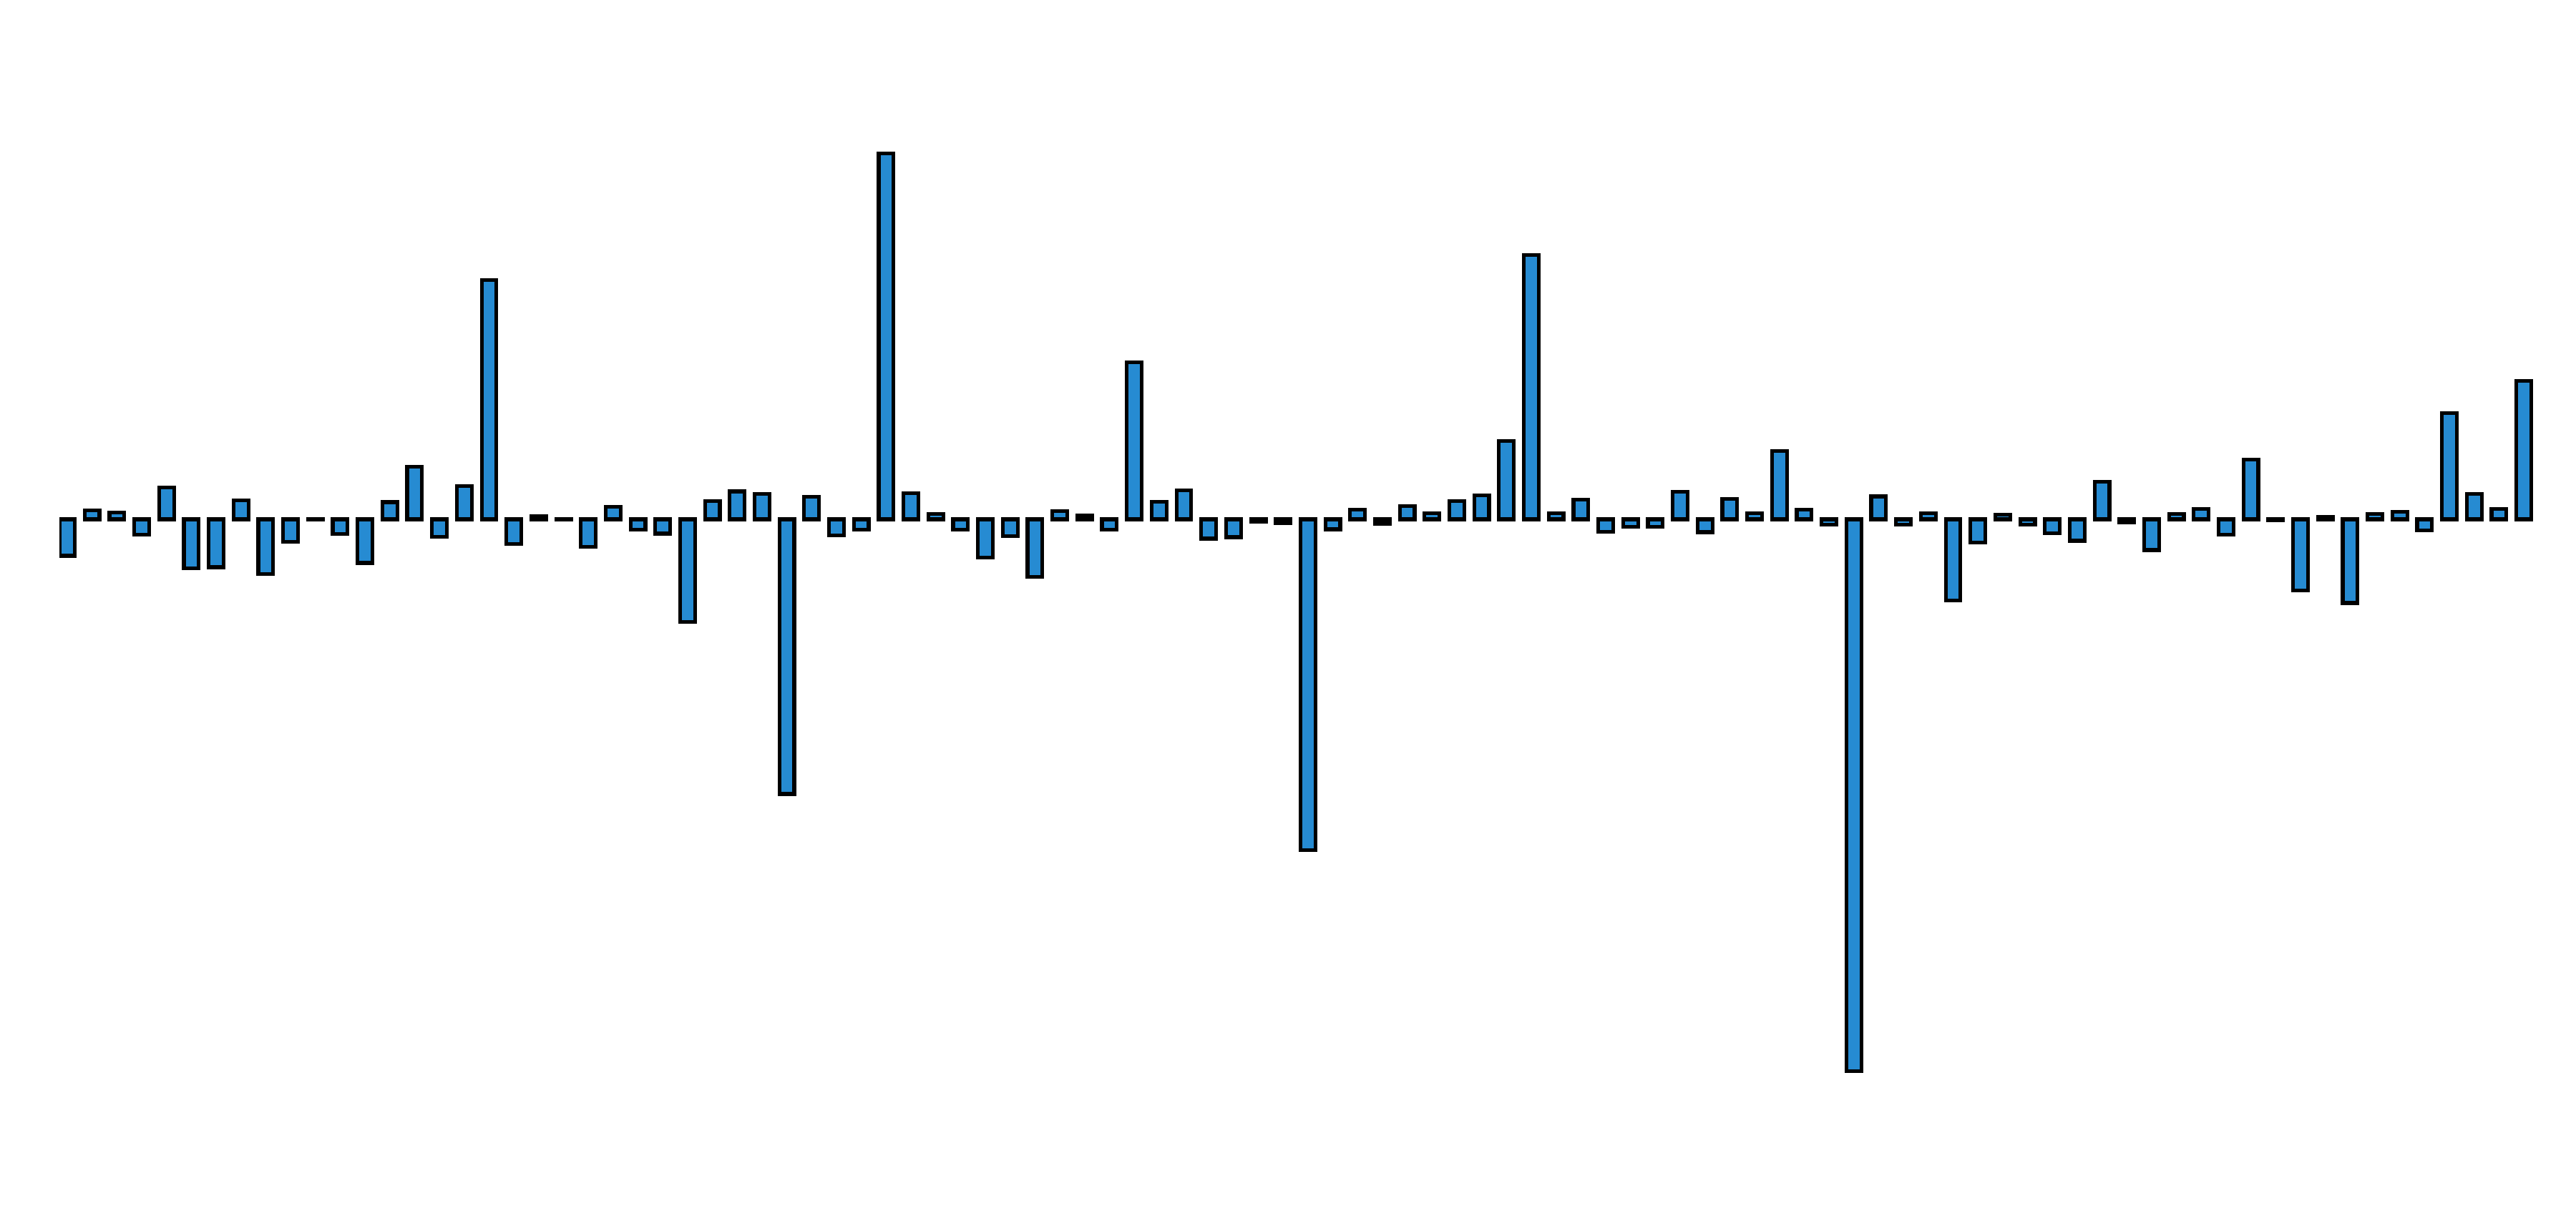
\includegraphics{LevyFlight/levy_length.pdf}
%     \end{center}
%     \caption{Distribution de 100 tirages aléatoire obéissant à une distribution de Lévy.
%              \label{fig:levy_length}}
% \end{figure}

% \begin{figure}
%     \begin{center}
%         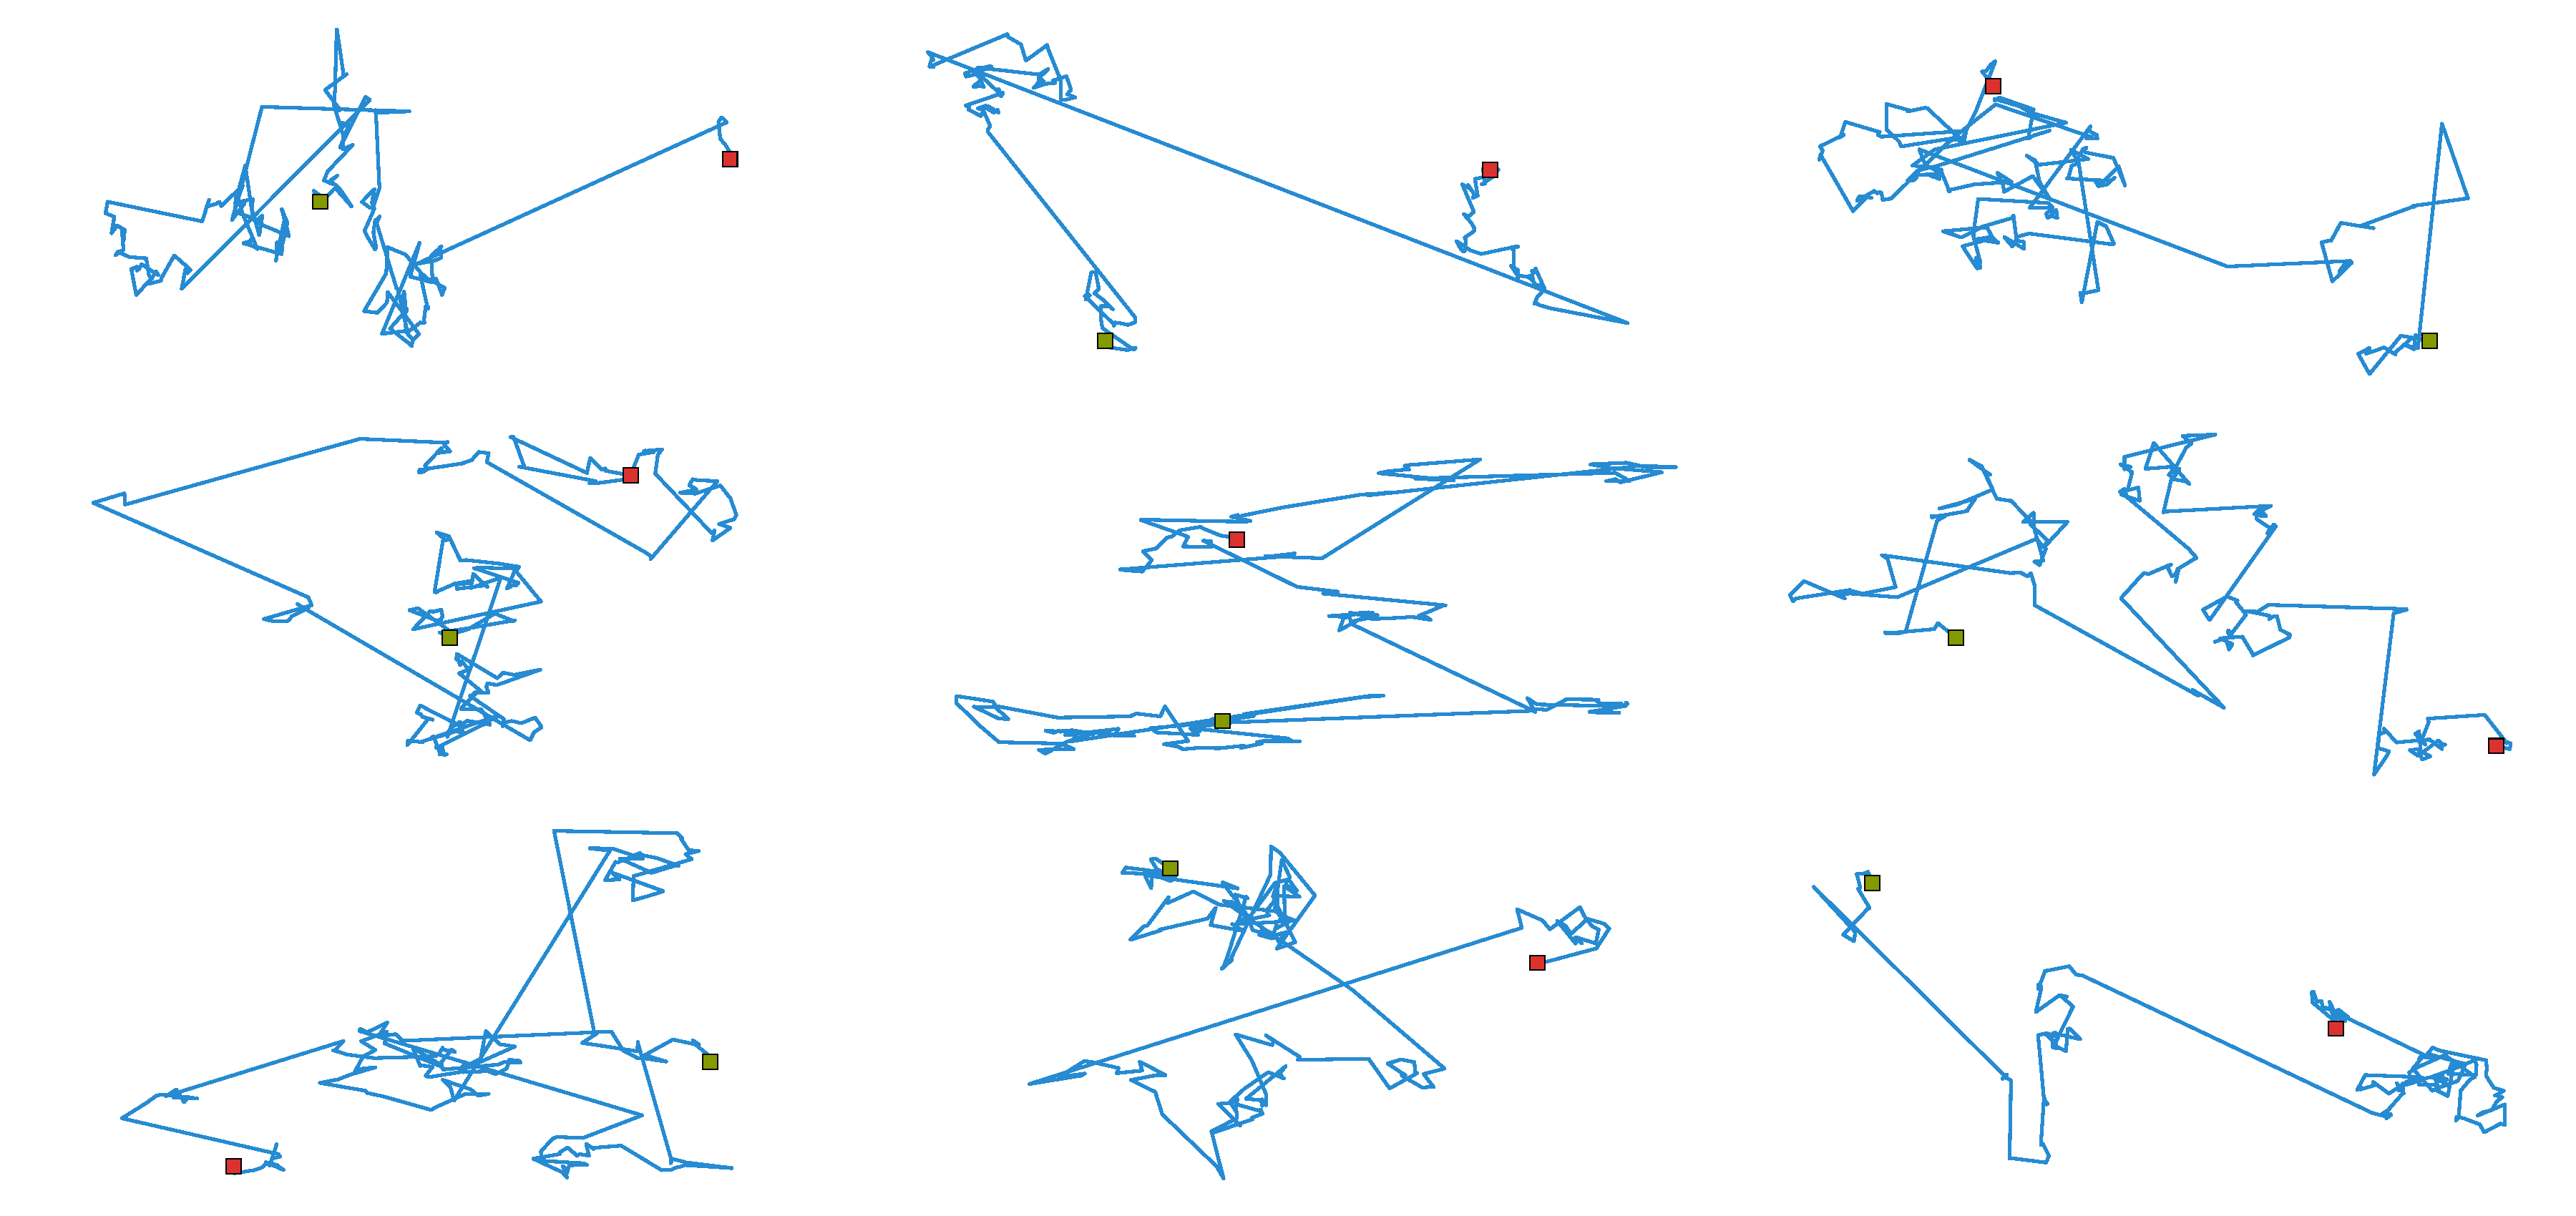
\includegraphics{LevyFlight/levy_flight.pdf}
%     \end{center}
%     \caption{Multiples vols de Lévy de 200 pas.
%              \label{fig:levy_flight}}
% \end{figure}

% \begin{figure}
%     \begin{center}
%         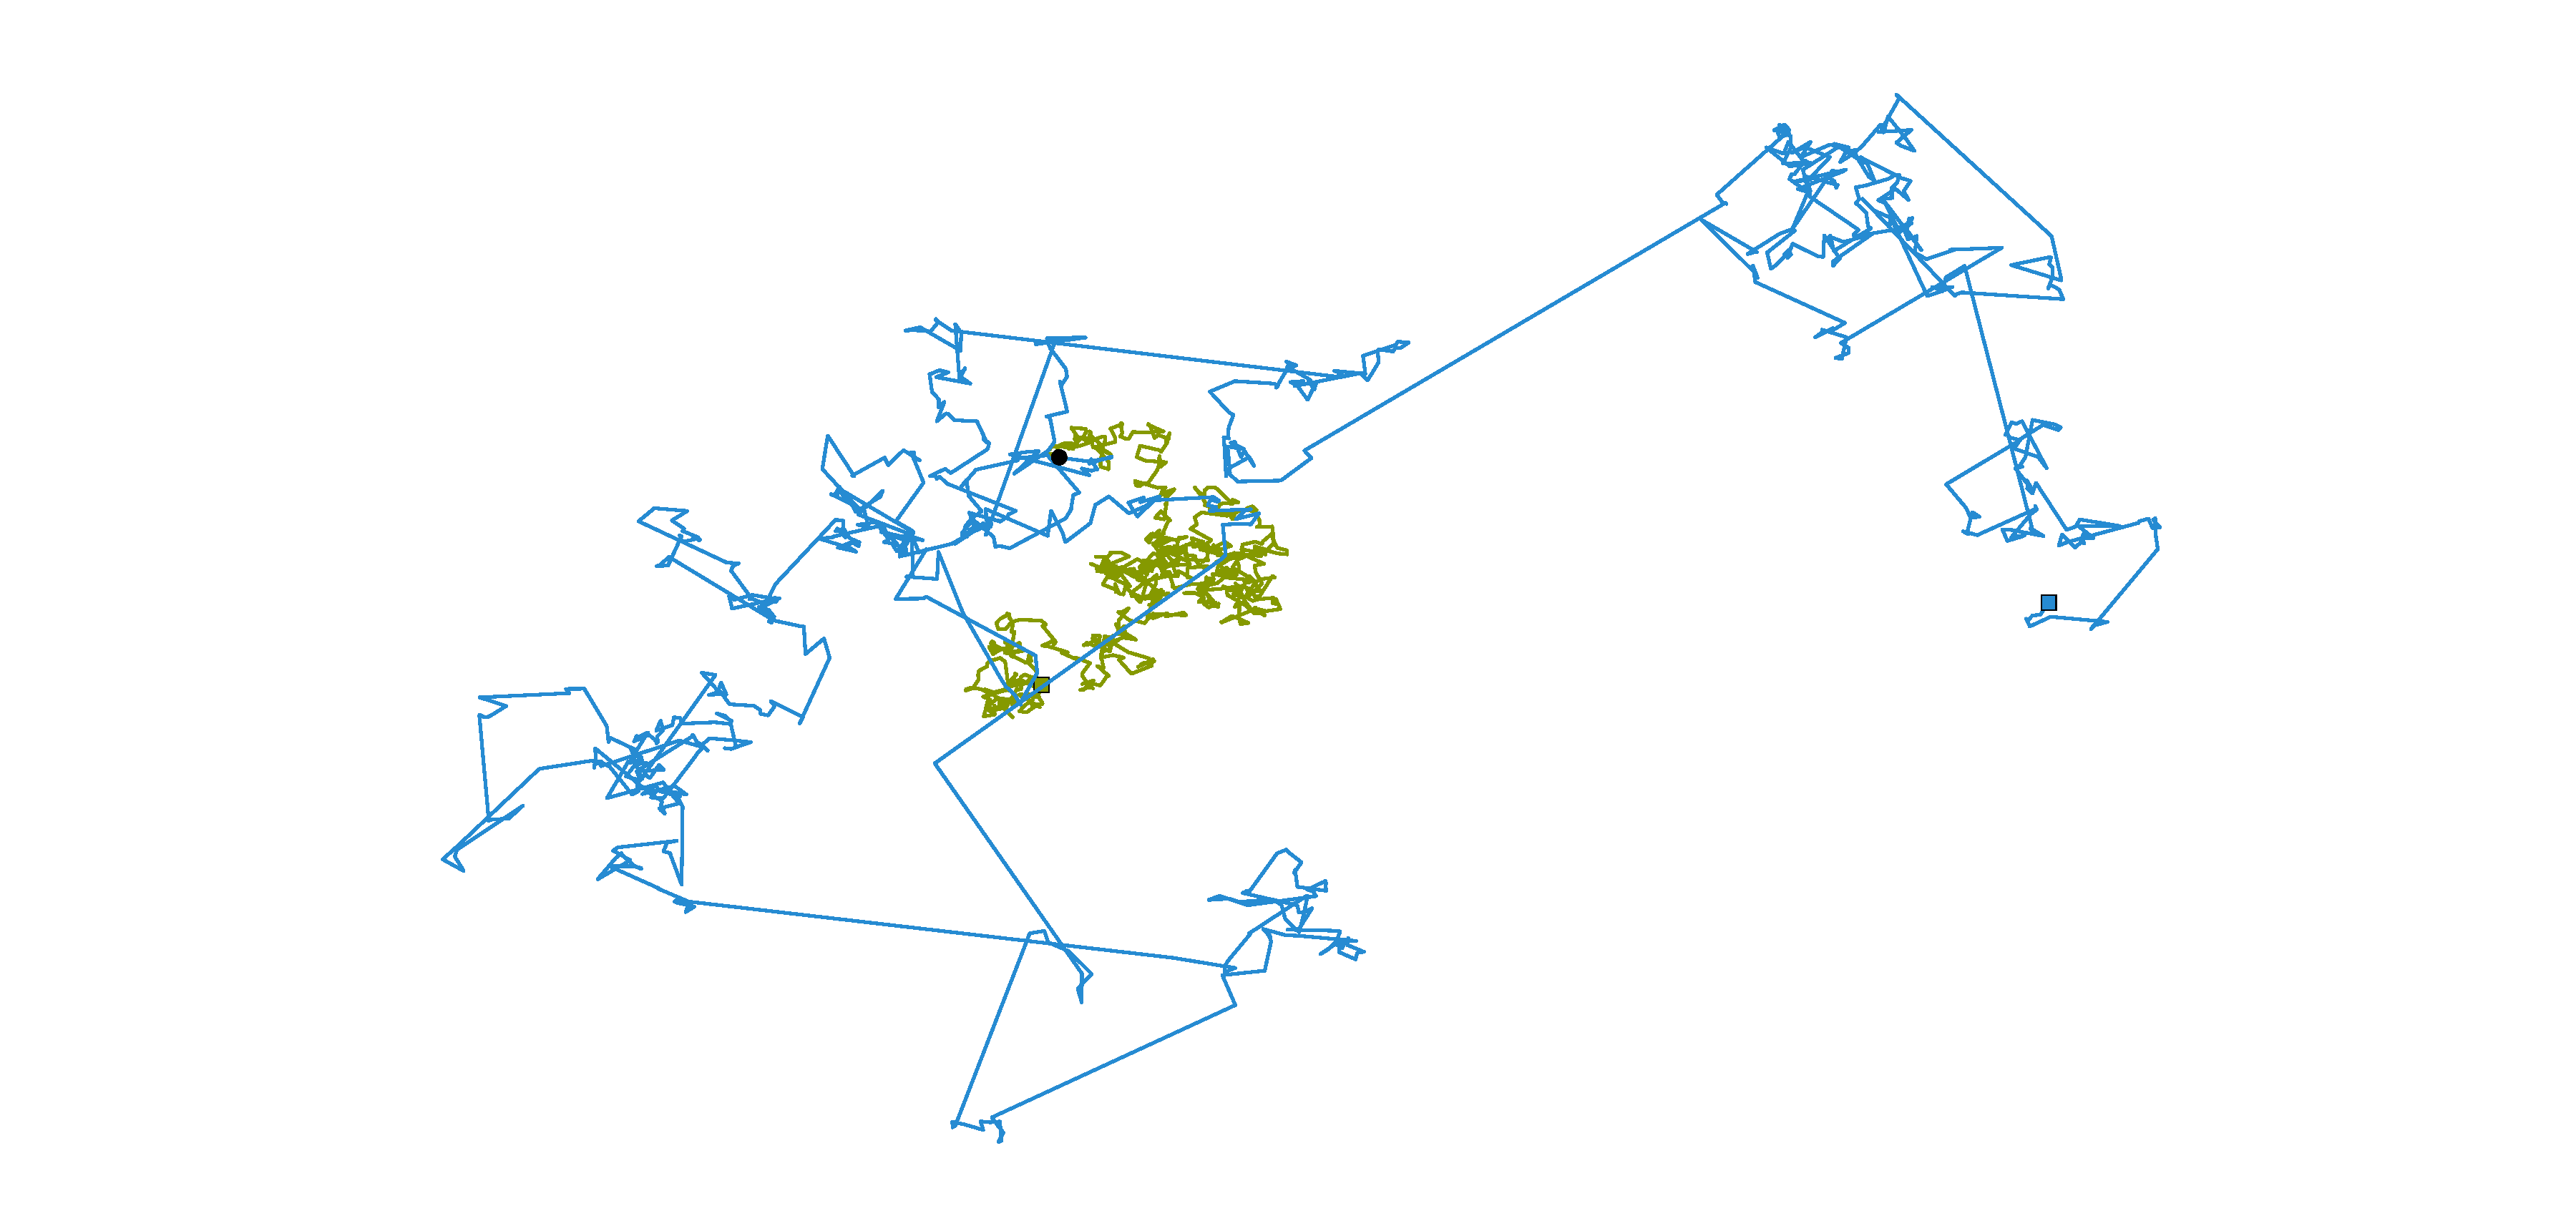
\includegraphics{LevyFlight/levy_vs_gaussian.pdf}
%     \end{center}
%     \caption{Mouvement browien (en vert) et vol de Lévy (en bleu) pour 200 pas aléatoires.
%              \label{fig:levy_vs_gaussian}}
% \end{figure}

% \itodo{Ajouter des applications aux problèmes multi-objectifs}
% Dans \cite{Sharma2012213}, vol de Lévy est employé pour améliorer l’algorithme ABC
% pour faire une recherche locale autour de la meilleure solution actuelle. L’auteur
% utilise un multiplicateur pour réduire la longueur des pas généré d’après \eqref{eq:step_len}.
% De plus la meilleure solution actuelle est utilisée pour guider la recherche aléatoire et
% peu être assimilé à un apprentissage. Le vol de Lévy a aussi été utilisé dans un algorithme
% d’optimisation approchée, le Cuckko search. Cet algorithme est inspiré du comportement
% parasitaire de la reproduction des cuculidés et a était adapté aux problèmes
% multi-objectifs \parencite{Yang20131616}).
% % subsubsection vol_de_lévy (end)

% % - - - - - - - - - - - - - - - - - - - - - - - - - - - - - - - - - - - - - - -
% \subsubsection{Apprentissage par opposition} % (fold)
% \label{ssub:apprentissage_par_opposition}

% La recherche par vecteur opposé (opposition-based learning) a été implémenté pour la première fois
% en optimisation par \cite{Tizhoosh2005695,Rahnamayan2008155}. Il propose une méthode permettant de diversifier la
% population sans connaissances à-priori.
% % Opposite based learning method
% \begin{Def}[OBLM~:~Opposition-Based Learning Method]\label{def:oblm}
% La recherche par vecteur opposé (Opposition-Based Learning) permet de diversifier la
% population sans connaissances à-priori.
% Admettons un point de dimension $D$, $P(x_{1}, x_{2}, ..., x_{D})$ avec
% $x_{1}, x_{2}, ..., x_{D}$ des valeurs bornées. Si $x_{i} \in [a_{i}, b_{i}]$ pour
% $i = 1, 2, ..., D$ alors le point opposée est $\check{P}(\check{x_{1}}, \check{x_{2}}, ..., \check{x_{D}})$ suivant:
% \[\check{x_{i}} = a_{i} + b_{i} - x_{i}\]
% \end{Def}

% Il est important de noter que les solutions sont comparées deux à deux par tournoi binaire, où
% seule la meilleure solution entre l’initiale et son opposée est conservée. Admettons une solution
% candidate $P(x_{1}, x_{2}, ..., x_{D})$ et son opposée $\check{P}(\check{x_{1}}, \check{x_{2}}, ..., \check{x_{D}})$,
% alors si $f(\check{P}) \geq f(P)$ alors la solution $P$ est remplacé par $\check{P}$.
% \ftodo{Illustration du tournoi binaire graphiquement}

% Cette méthode a ensuite été améliorée \parencite{Rahnamayan2008155}) puis adaptée à
% l’algorithme Differential evolution (DE). La méthode reprend la définition de base
% mais définit plus clairement les limites et la portée de la méthode.
% La méthode est utilisée durant la phase d’initialisation pour améliorer la diversité
% en générant une population aléatoire de $n$ individus puis $n$ opposées.
% Les solutions les plus performantes étant ensuite conservées pour obtenir une population
% finale de $n$ individus.
% Ensuite durant l’exécution de l’algorithme de nouvelles populations opposées sont générées.
% Un coefficient $J_r$ est utilisé pour contrôler la probabilité de générer cette nouvelle
% population opposée pour chaque itération.

% La méthode a ensuite été testée sur un jeu de 15 fonctions de références (7 uni-modales
% et 8 multi-modales). La nouvelle approche permet alors de trouver de meilleurs
% résultats sur 14 des 15 fonctions. Il est aussi montré la supériorité de la
% sélection par opposition par rapport au caractère aléatoire \parencite{Rahnamayan2008155,Rahnamayan2008906})
% Il est aussi mis en avant que la probabilité de générer une population opposée
% doit décroitre au fur et à mesure des itérations. En effet, la méthode permet de
% réduire l’espace de recherche mais ralenti la convergence une fois cette intervalle
% faible. Finalement il est proposé une intervalle de performance pour le coefficient si le problème
% ne permet pas de déterminer un nombre fixe d’itération à-priori: $[0.1 < J_r < 0.4]$.

% Cette approche a été appliquée avec succès dans le cas de l’algorithme ABC en couplage
% avec un opérateur de mutation \parencite{Bi2011174}) ou encore en coopération avec une marche
% aléatoire \parencite{Sharma2012213}).
% Il a aussi été appliqué pour résoudre des problèmes plus complexe à objectifs multiples,
% en combinaison avec un algorithme évolutionnaire \parencite{Ma201448}), ou encore avec le PSO \parencite{Gao2013114}).

% Notre problème ne nous permettant pas d’avoir de connaissance à-priori, il nous est
% impossible d’estimer le nombre d’itération nécessaires et l’utilisation d’un coefficient $J_r$
% dynamique difficile.
% % Au vu des recommandations et des applications déjà faites pour des problèmes mono-critères,
% % ce coefficient sera fixé à 0.1 dans un premier temps.

% \begin{figure}
%     \begin{center}
%         \includegraphics{abc/principe_obl.pdf}
%     \end{center}
%     \caption{Principe de fonctionnement de la recherche par vecteur opposée.
%              \label{fig:OBL_method}}
% \end{figure}
% % subsubsection apprentissage_par_opposition (end)
% % subsection ameliorer_l_exploration_et_l_exploitation (end)


% % ------------------------------------------------------------------------------
% \subsection{Prendre en compte les contraintes: quelle méthode ?} % (fold)
% \label{sub:prendre_en_compte_les_contraintes_quelle_methode}
% \itodo{Décrire les approches pour tacler les problèmes avec contraintes.
%        Homorphous mapping, assimilation à un autre objectif (Voir Karaboga20113021)}

% De nombreuses améliorations ont été proposées pour améliorer la vitesse de convergence
% vers le ou les optimaux tout en évitant les optimums locaux. Cependant dans certaines
% optimisation les objectifs sont dépendant de contraintes. Dans certaines conditions, il
% est possible de résoudre ce problème de contrainte en bornant les variables à des solutions
% réalisables mais ce n’est pas toujours possible. Lorsque ces contraintes ne peuvent pas être vérifiées
% en amont de l’optimisation, il faut alors en tenir compte durant ce processus à l’aide
% de méthode plus ou moins complexes.

% La pénalité est l’approche la plus souvent retenue \parencite{EfrEnMezura-Montes2003}\munsure{Peut être mettre un vrai article ?}).
% Cette approche demande la définition d’un facteur de pénalité qui doit être définie
% avec précision pour pouvoir converger vers le/les solutions optimales qui respectent les
% contraintes. Ce paramètre est dit: (i) statique si la pénalité est la somme pondérée des contraintes,
% (ii) dynamique si le nombre d’itération influence le paramètre, (iii) adaptatif si l’information de la
% recherche aide à sa détermination \parencite{Woldesenbet20073077}.
% Enfin il est important de noter que une solution respectant toutes les contraintes sera toujours préférée
% à une solution violant des contraintes même si l’évaluation des objectifs est meilleur. Il peut ainsi être
% difficile d’atteindre certaines optimums\mtodo{Ceux qui sont entourés de violeur de contraintes} particulièrement
% dans un espace de solutions faisables limitée.
% \cite{Tsai201480} l’utilise avec deux essaims d’abeilles respectant respectivement l’algorithme
% ABC et l’algorithme Bee Algorithm (BA) avec une population ajustée dynamiquement ou encore \cite{Karaboga20113021}
% qui autorise des solutions ne respectant pas les contraintes à être ajoutées à la population. Ce dernier
% utilise une facteur de pénalité déterminer dynamiquement évitant sa détermination empiriquement
% \parencite{Deb2000311}\mtodo{Lire cet article !!} comme les approches plus classiques de pénalité.
% \\

% \cite{EfrEnMezura-Montes2003} propose une méthode basée sur la sélection par tournoi binaire couplé à un mécanisme
% déterministe permettant d’accepter des solutions infaisables. La probabilité de sélectionner une solution
% seulement sur la performance des fonctions objectifs évolue est un paramètre adaptatif. Si durant une
% certaine intervalle la déviation moyenne évolue faiblement alors la probabilité de pouvoir sélectionner
% une solution uniquement sur optimalité des objectifs augmente et inversement.


% \cite{Woldesenbet20073077} propose aussi une méthode ne demandant pas de paramètres supplémentaires
% qui doivent être déterminé empiriquement. La première étape est de normalisé les objectifs et contraintes
% grâce aux minimums et maximums à chaque itération. Ensuite une distance $d_{i}$ est
% évaluée et la distance minimale est conservée. Soit $\tilde{f}$ respectivement la fonction objectif $i$ normalisée
% et la somme des contraintes normalisées alors la distance s’écrit:
% \begin{align}\label{eq:distance_measure}
%     d_{i} = \begin{cases}
%                 v(x),                               \qquad & if\  r_{f} = 0\\
%                 \sqrt{\tilde{f}(x)^{2} + v(x)^{2}}, \qquad & otherwise\\
%             \end{cases}
% \end{align}
% avec:
% \begin{equation*}
%     r_{f} = \frac{\text{Nbr de solutions faisable dans la population}}{\text{Taille de la population}}
% \end{equation*}
% Afin d’orienter la recherche vers un espace de solution faisables, une pénalité adaptative
% est utilisé, $p_{i}(x)$, donnant un objectif final modifié de la forme: $F_{i}(x) = d_{i}(x) + p_{i}(x)$.
% La population peut ainsi accepter des solutions ne respectant pas les contraintes mais
% l’archive (optimisation multi-objectifs) elle n’accepte que des solutions faisables.
% % subsection prendre_en_compte_les_contraintes_quelle_methode (end)


% % ------------------------------------------------------------------------------
% \subsection{Vers un outil d’aide à la décision par optimisation multi-objectif} % (fold)
% \label{sub:vers_un_outil_d_aide_à_la_décision_par_optimisation_multi_objectif}
% \itodo{Ajouter une vision globale du processus d’optimisation sous forme de graphique
%       servant de résumé du chapitre.}

% L’algorithme ABC modifié (Fig.~\ref{fig:abc_modifie}) comprend les même phases que l’original. La différence réside
% dans le déroulement de ces phases. En effet plusieurs technique présentées ci-avant
% ont été implémentées afin d’améliorer l’exploitation et l’exploration de l’algorithme.
% Enfin une archive par $\epsilon$-dominance est utilisé pour maintenir les solutions
% non-dominées formant le front de Pareto. Cette archive est mise à jour après chaque
% évaluation contrairement aux sources qui ne sont mis à jour que après chaque phase.

% \begin{figure}
%     \begin{center}
%         \includegraphics[width=10cm, height=15cm]{abc/algorithme_complet.png}
%     \end{center}
%     \caption{Description globale de l’algorithme ABC modifié. Chaque phase renvois à un algorithme.
%              \label{fig:abc_modifie}}
% \end{figure}

% Dans un premier temps l’algorithme initialise l’archive grâce aux objectifs et aux valeurs
% d’epsilons puis la population est initialisé aléatoirement par OBL afin d’obtenir une meilleure diversité
% (Algorithm~\ref{alg:init_phase}). Ensuite on entre dans le processus itératif
% tant que la ou les conditions d’arrêts ne sont pas atteintes. Les différentes phases
% sont les suivantes: (i) Phase des butineuses (Algorithm~\ref{alg:employed_phase}) qui explore l’espace de décision avec des vols de
% Lévy, (ii) Phase des ouvrières (Algorithm~\ref{alg:onlooker_phase}) qui utilisent les informations acquises par les butineuses
% et améliorent les sources choisies \eqref{eq:attribution_prob_to_source}, (iii) Phase des éclaireuses
% (Algorithm~\ref{alg:scout_phase}) qui réinitialisent une source si elle est non fructueuse.

% La longueur du vol de Lévy est définie par:
% \begin{equation}\label{eq:levy_flight}
%   LevyFlight = scaleFactor \times stepLength \times RandUniform(0, 1)
% \end{equation}
% avec $stepLength$ définie par \eqref{eq:step_len} et $scaleFactor$ fixé à 0.01.\\


% % Attribution des probabilités
% La probabilité de choisir une source $k$ par une ouvrière est elle définie comme:
% \begin{subequations}\label{eq:attribution_prob_to_source}
%   \begin{align}
%     prob_{k} = &\frac{Qualite(\vec{x}_{k})}{\sum_{i=1}^{NbrSources} Qualite(\vec{x}_{i})} \\[1em]
%     Qualite(\vec{x}_{k}) = &\frac{Dominance(k)}{NbrSources}
%   \end{align}
%   avec \emph{Dominance(k)} le nombre de source que la source $k$ domine, et \emph{Fitness}
%   la qualité de la source en tenant comptes des contraintes comme définies en.
% \end{subequations}

% % Phase d’initialisation
% \begin{algorithm}\label{alg:init_phase}
%   \SetAlgoVlined
%   \emph{Initialisation des sources sur l’ensemble de l’espace de décision}\;
%   \For{$i \leftarrow 0$ \KwTo \ANbrSources}
%   {
%     \emph{Initialisation des critères pour chaque source}\;
%     \For{$j \leftarrow 0$ \KwTo \ANbrCriteria}
%     {
%       \AComment{Génération aléatoire de la position initiale}
%       $x_{ij} = x_{j}^{min} + RandUniform(0, 1) \times (x_{j}^{max} - x_{j}^{min})$\;
%       avec $RandUniform$ un tirage aléatoire suivant une loi uniforme, et $x_{j}^{min}$, $x_{j}^{max}$
%       respectivement le minimum et le maximum du critère $j$\;
      \BlankLine
%       \AComment{Génération de la position opposée suivant Définition~\ref{def:oblm}}
%       $ \check{x_{ij}} = a_{j} + b_{j} - x_{ij}$\;
%       avec $a_{j}$, $b_{j}$ respectivement les bornes inférieures et supérieurs du critère
%     }
%     \If{$\ASource_{i}$ respecte toutes les contraintes}
%     {
%       \AComment{On ajoute la source initial à l’archive}
%       $\AArchive \pluseq \ASource_{i}$\;
%     }
%     \If{$\check{\ASource_{i}}$ respecte toutes les contraintes}
%     {
%       \AComment{On ajoute la source opposée à l’archive}
%       $\AArchive \pluseq \check{\ASource_{i}}$\;
%     }
%   }
%   \AComment{On ne conserve que une seule position par source}
%   Mise à jour de la position des \ASources d’après Algorithm~\ref{alg:maj_phase}\;
%   \caption{Initialisation des sources par OBLM (Opposite-Based Learning Method).}
% \end{algorithm}

% % Maj des sources
% \begin{algorithm}\label{alg:maj_phase}
%   \SetAlgoVlined
%   Récupérer le maximum et minimum pour chaque objectif\;
%   Récupérer le maximum pour chaque contrainte\;
%   \For{$i \leftarrow 0$ \KwTo \ANbrSources}
%   {
%     Normaliser les objectifs et les contraintes avec ()\;
%     Calculer la valeur de distance $\vec{d_{i}}$ en utilisant \eqref{eq:distance_measure}\;
%     Calculer la pénalité $\vec{p_{i}}$ d’après ()\;
%     \AComment{Attribuer les nouvelles valeurs d’objectifs aux sources}
%     $\vec{F_{i}} = \vec{d_{i}} + \vec{p_{i}}$\;
%     \If{$\check{\vec{F_{i}}} \succ \vec{F_{i}}$}
%     {
%       \AComment{On remplace la position de la source par la nouvelle}
%       $\vec{x_{i}} \leftarrow \check{\vec{x_{i}}}$\;
%       \AComment{On réinitialise le nombre d’échec pour la source $i$}
%       $\ATrial_{i} \leftarrow 0$\;
%     }
%     \Else
%     {
%       \AComment{On incrémente le nombre d’échec pour la source $i$}
%       $\ATrial_{i} \pluseq 1$\;
%     }
%     avec $\vec{F_{i}}$, $\check{\vec{F_{i}}}$ respectivement les vecteurs objectifs
%     normalisés pour l’ancienne et la nouvelle position.\;
%   }
%   \caption{Mise à jour des sources}
% \end{algorithm}

% % Phase des butineuses
% \begin{algorithm}\label{alg:employed_phase}
%   \SetAlgoVlined
%   \AComment{Exploration des sources par les \AEmployed}
%   \For{$i \leftarrow 0$ \KwTo \ANbrSources}
%   {
%     Sélection aléatoire d’une source $k$ dans l’\AArchive\;
%     \AComment{Génération d’une nouvelle position pour la \ASource $i$}
%     \For{$j \leftarrow 0$ \KwTo \ANbrCriteria}
%     {
%       \begin{algomathdisplay}
%         \check{x_{ij}} =%
%           \begin{cases}
%             x_{ij} + \ALevyFlight_{ij} \times (x_{ij} - x_{kj}) &\ \ATirage < \AMR \\
%             x_{ij}                                      &\ sinon
%           \end{cases}
%       \end{algomathdisplay}
%       avec \ATirage un nombre aléatoire uniforme (entre 0 et 1),
%       \AMR un paramètre contrôlant le nombre de modifications
%       et \ALevyFlight définie par \eqref{eq:levy_flight}\;
%     }
%     \If{aucun critère n’a été modifié}
%       {
%         \AComment{Sélection aléatoire d’un critère $j$ à mettre à jour}
%         $\check{x_{ij}} = x_{ij} + \ALevyFlight_{ij} \times (x_{ij} - x_{kj})$\;
%       }
%     \If{$\ASource_{i}$ respecte toutes les contraintes}
%     {
%       \AComment{On ajoute la source initial à l’archive}
%       $\AArchive \pluseq \ASource_{i}$\;
%     }
%     \If{$\check{\ASource_{i}}$ respecte toutes les contraintes}
%     {
%       \AComment{On ajoute la source opposée à l’archive}
%       $\AArchive \pluseq \check{\ASource_{i}}$\;
%     }
%   }
%   \AComment{On ne conserve que une seule position par source}
%   Mise à jour de la position des \ASources d’après Algorithm~\ref{alg:maj_phase}\;
%   \caption{Phase des butineuses.}
% \end{algorithm}

% % Phase des ouvrières
% \begin{algorithm}\label{alg:onlooker_phase}
%   \SetAlgoVlined
%   \AComment{Exploitation des sources par les \AOnlookers}
%   \For{$\ABee \in \AOnlookers$}
%     {
%       Sélection aléatoire d’une \ASource $i$ selon la probabilité
%       définie par l’équation \eqref{eq:attribution_prob_to_source} (Sélection par roulette)\;
%       Génération d’une nouvelle position pour la \ASource $i$ selon Algorithm~\ref{alg:employed_phase}
%       (lignes 3 à 16)\;
%     }
%   \AComment{On ne conserve que une seule position par source}
%   \AComment{Plusieurs \AOnlookers peuvent modifier la même source}
%   Mise à jour de la position des \ASources qui ont été modifiées d’après Algorithm~\ref{alg:maj_phase}\;
%   \caption{Phase des ouvrières.}
% \end{algorithm}

% % Phase des éclaireuses
% \begin{algorithm}\label{alg:scout_phase}
%   \SetAlgoVlined
%   \For{$i \leftarrow 0$ \KwTo \ANbrSources}
%   {
%     \If{$\ATrial_{i} > \AMaxTrial$ }
%     {
%       \AComment{Exploration par les \AScouts}
%       Génération de deux nouvelles positions suivant Algorithm~\ref{alg:init_phase}
%       (lignes 4 à 16)\;
%     }
%   }
%   \AComment{On conserve la meilleure solution parmi les deux nouvelles}
%   Mise à jour de la position des \ASources d’après Algorithm~\ref{alg:maj_phase}\;
%   \caption{Phase des éclaireuses.}
% \end{algorithm}
% % subsection vers_un_outil_d_aide_à_la_décision_par_optimisation_multi_objectif (end)
% % section construction_d_un_outil_d_aide_à_la_decision (end)
